\chapter{Implementasjon}
Dette kapittelet tar for seg resultatet av utformingen av applikasjonen, hvordan tilstandshåndteringen er implementert og hvordan applikasjonen samhandler med backendløsningen i Firebase. Det ble tidlig besluttet å ikke utføre brukertester på prototypedesignet som ble laget i Figma. Årsaken til dette var at det ble sett på som lite hensiktsmessig da applikasjonen i stor grad ville ta i bruk funksjonalitet som ikke kunne testes i prototypeverktøyet. Her tenkes det spesifikt på bruk av kart og GPS, som er en av hovedfunksjonalitetene i applikasjonen. Implementasjonen ble derfor startet på direkte etter at prototypedesignet i Figma var ferdigstilt.

\section{Utforming}
Dette underkapittelet tar for seg resultatene av utformingen av selve applikasjonen. De forskjellige brukergrensesnitt-sidene er utviklet i henhold til prototype-designet (se kapittel \ref{cha:Design} \nameref{cha:Design}) som ble laget i Figma under design-fasen av prosjektet. Alle figurene vist i dette underkapittelet er skjermbilder hentet fra iOS-versjonen av applikasjonen på iPhone 12 Pro. 

\subsection{Login}
Login-siden er den eneste siden som ikke har et prototype-design laget i Figma. Dette er fordi det først var tenkt å bruke et ferdiglaget verktøy for implementering av brukergrensesnitt for innloggingsider i Angular med Firebase kalt FirebaseUI-Angular \cite{jenniRaphaelJenniFirebaseUIAngular2021}. Grunnet problemer under implementasjonen av FirebaseUI-Angular ble denne idéen skrinlagt og en standard login-side med bruk av e-post og passord ble utformet isteden. Logikken og funksjonaliteten rundt selve innloggingen blir forklart i underkapittel \ref{sub:backend-login} \nameref{sub:backend-login}.
\begin{figure}[H]
\centering
\captionsetup{width=.8\linewidth}
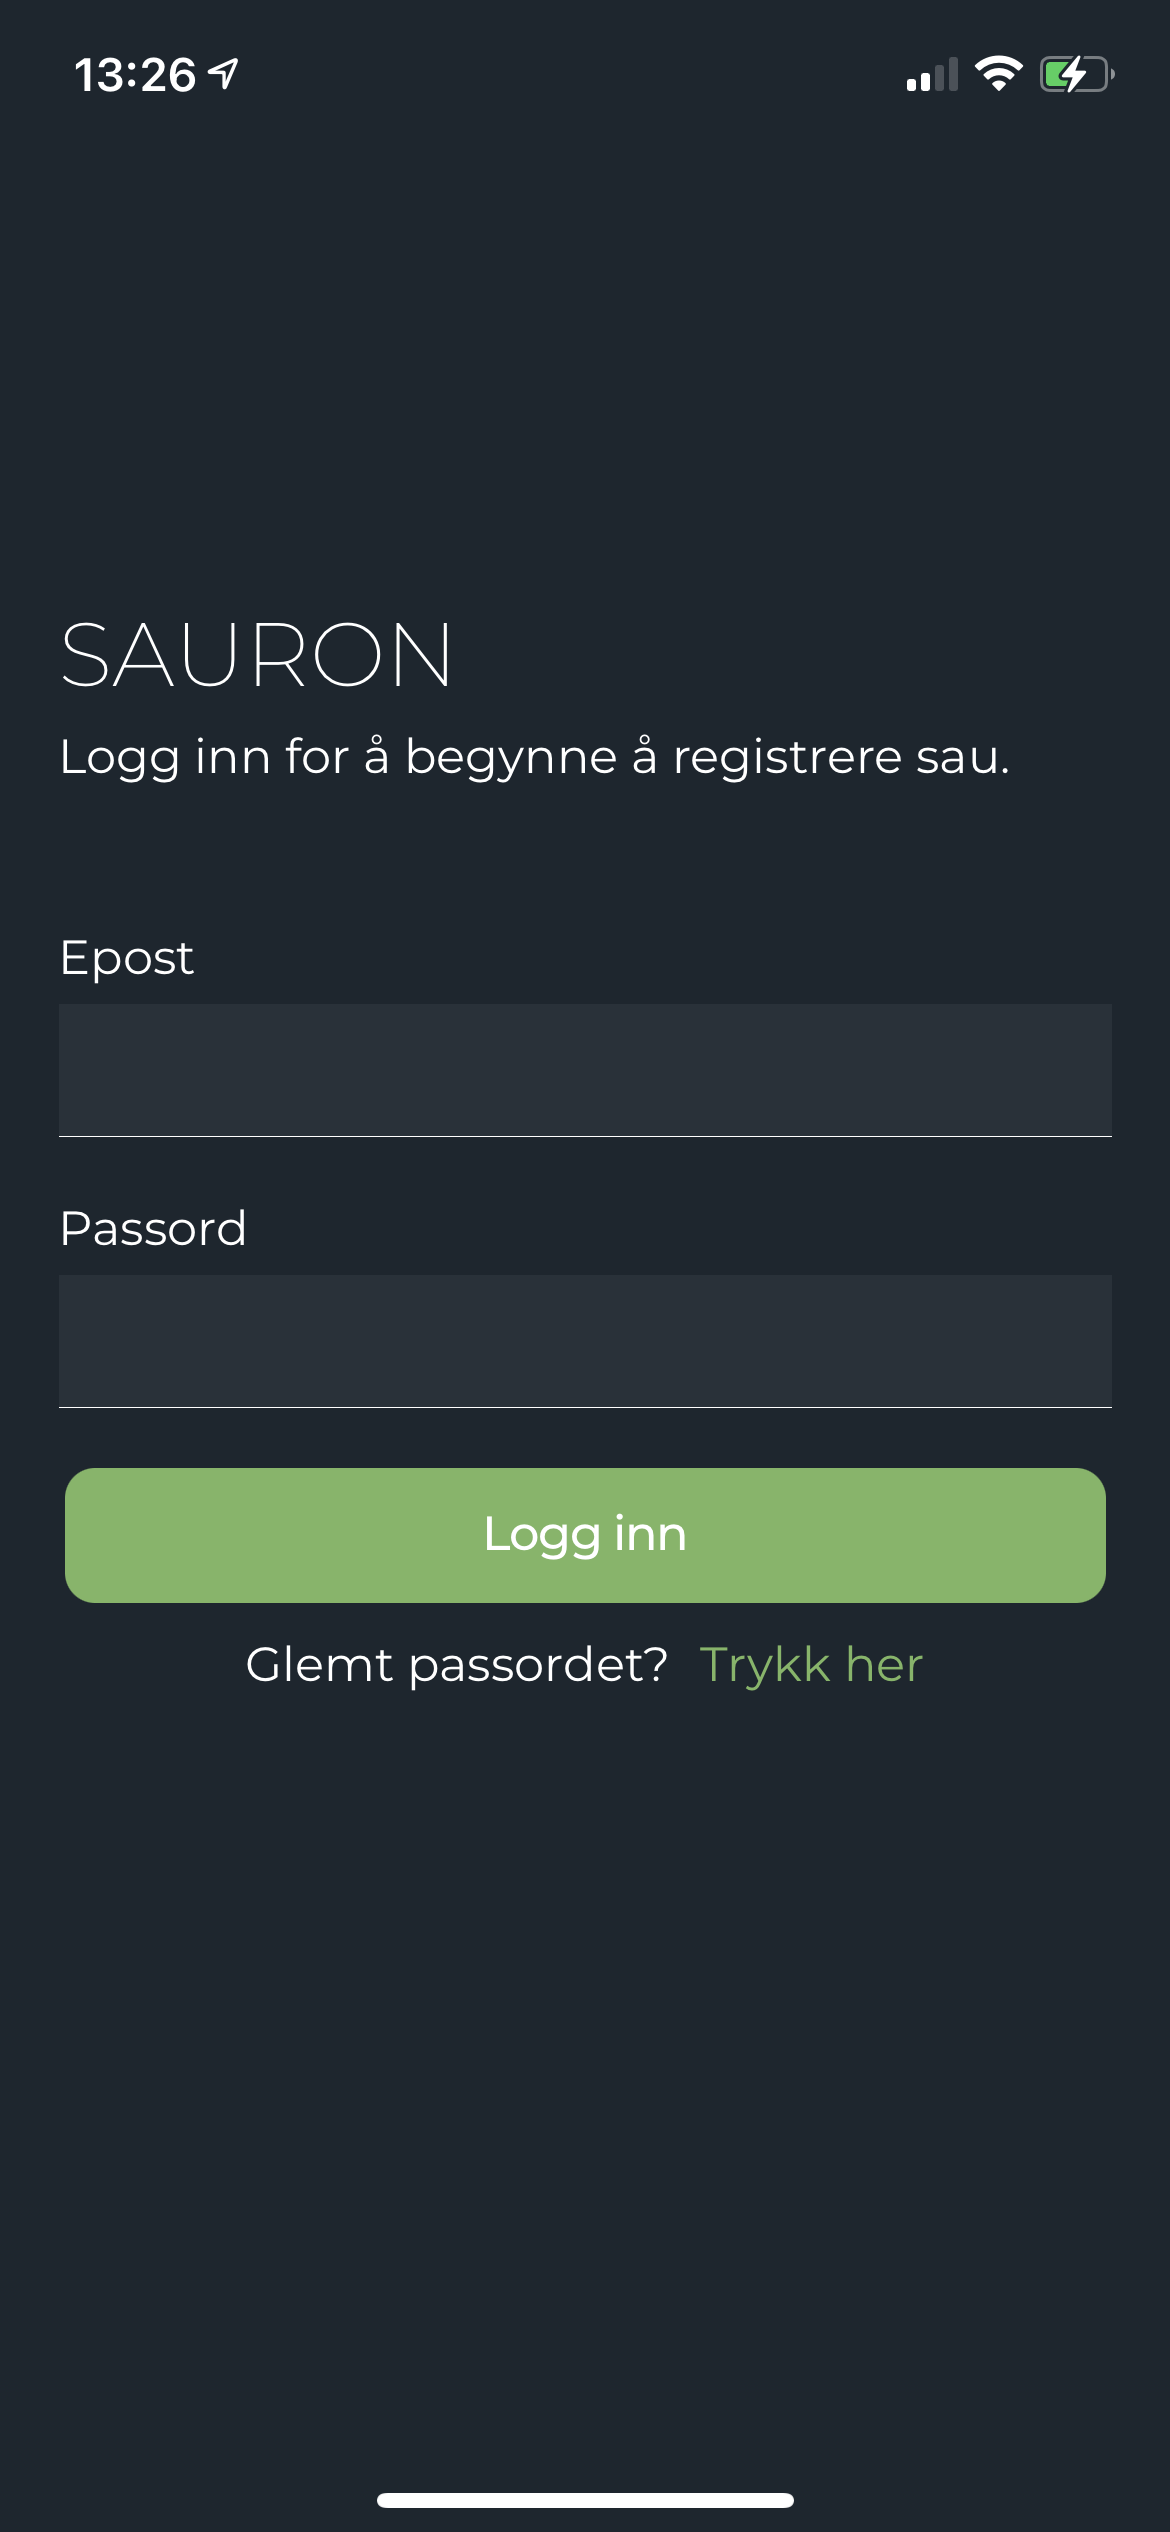
\includegraphics[scale=0.4]{Figurer/skjermbilder/login.png}
\caption{Login-side for applikasjonen.}
\label{fig:login}
\end{figure}

\subsection{Nedlasting av kartutsnitt}
\subsubsection{Oversikt over nedlastede kartutsnitt}
Siden som viser en liste over alle nedlastede kartutsnitt er utformet i henhold til design-prototypen. Det samme gjelder for valgmenyen som kommer opp hvis man trykker på de tre prikkene til høyre for hvert liste-element. Under intern testing av grensesnittet viste det seg at det var behov for en navigasjonsknapp for å kunne navigere tilbake til hovedmenyen om ønskelig. Denne har blitt implementert i form av en pil som peker til venstre opp i venstre hjørne av grensesnittet (se figur \ref{fig:nedlastede-kartutsnitt}). 
\begin{figure}[H]
  \centering
  \begin{minipage}[b]{0.4\textwidth}
    \centering
    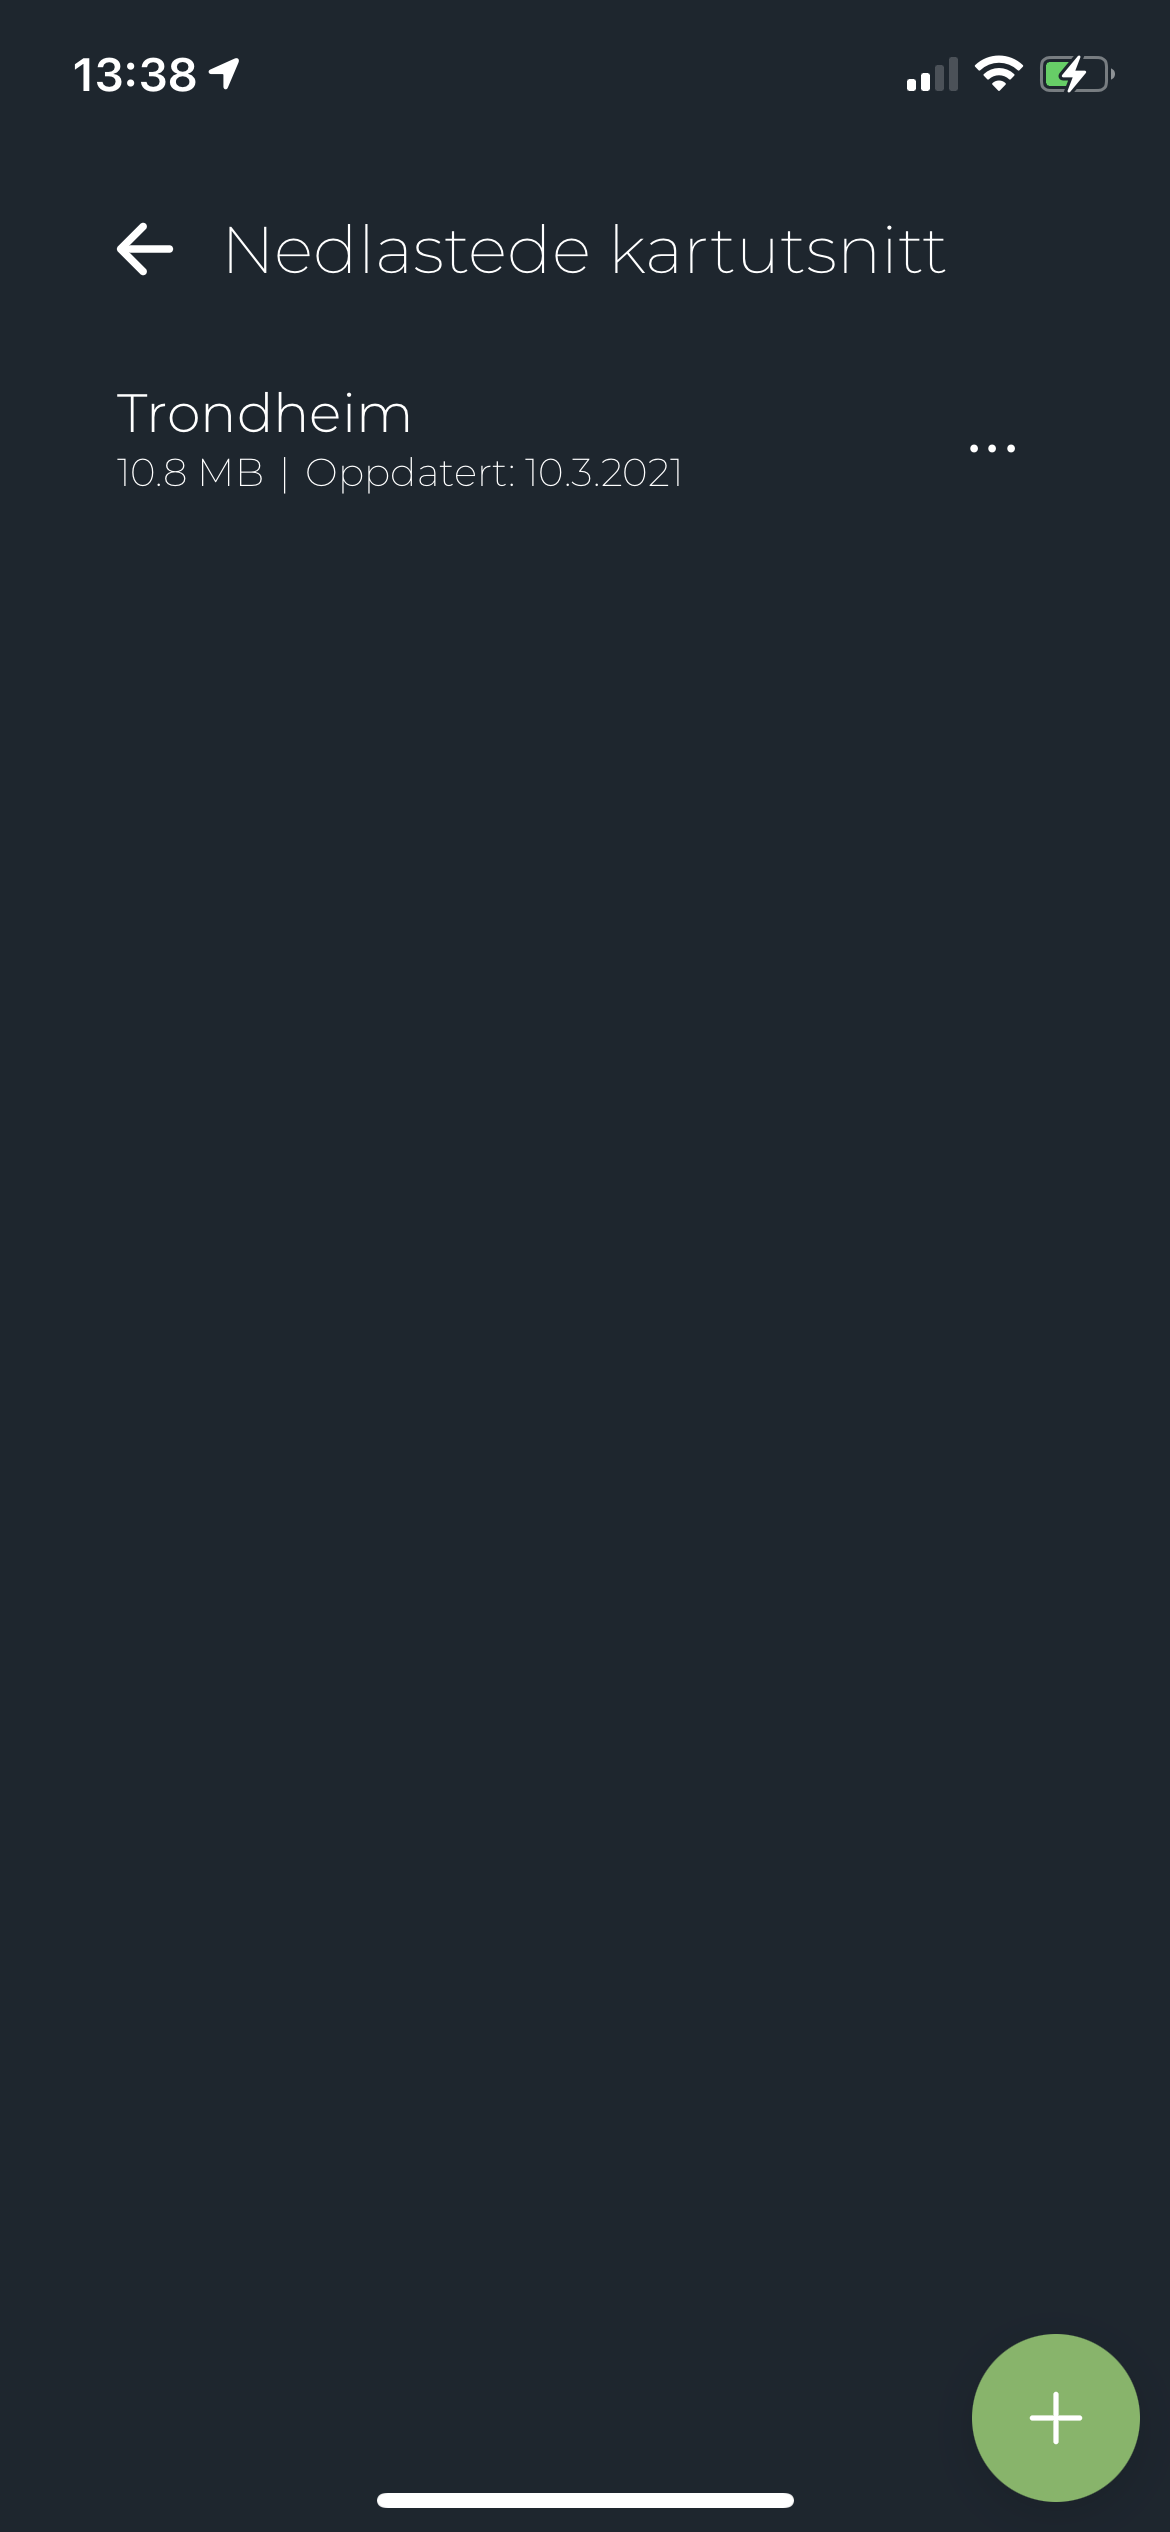
\includegraphics[scale=0.4]{Figurer/skjermbilder/nedlastede-kartutsnitt.png}
    \caption{Oversikt over nedlastede kartutsnitt.}
    \label{fig:nedlastede-kartutsnitt}
  \end{minipage}
  \hfill
  \begin{minipage}[b]{0.4\textwidth}
    \centering
    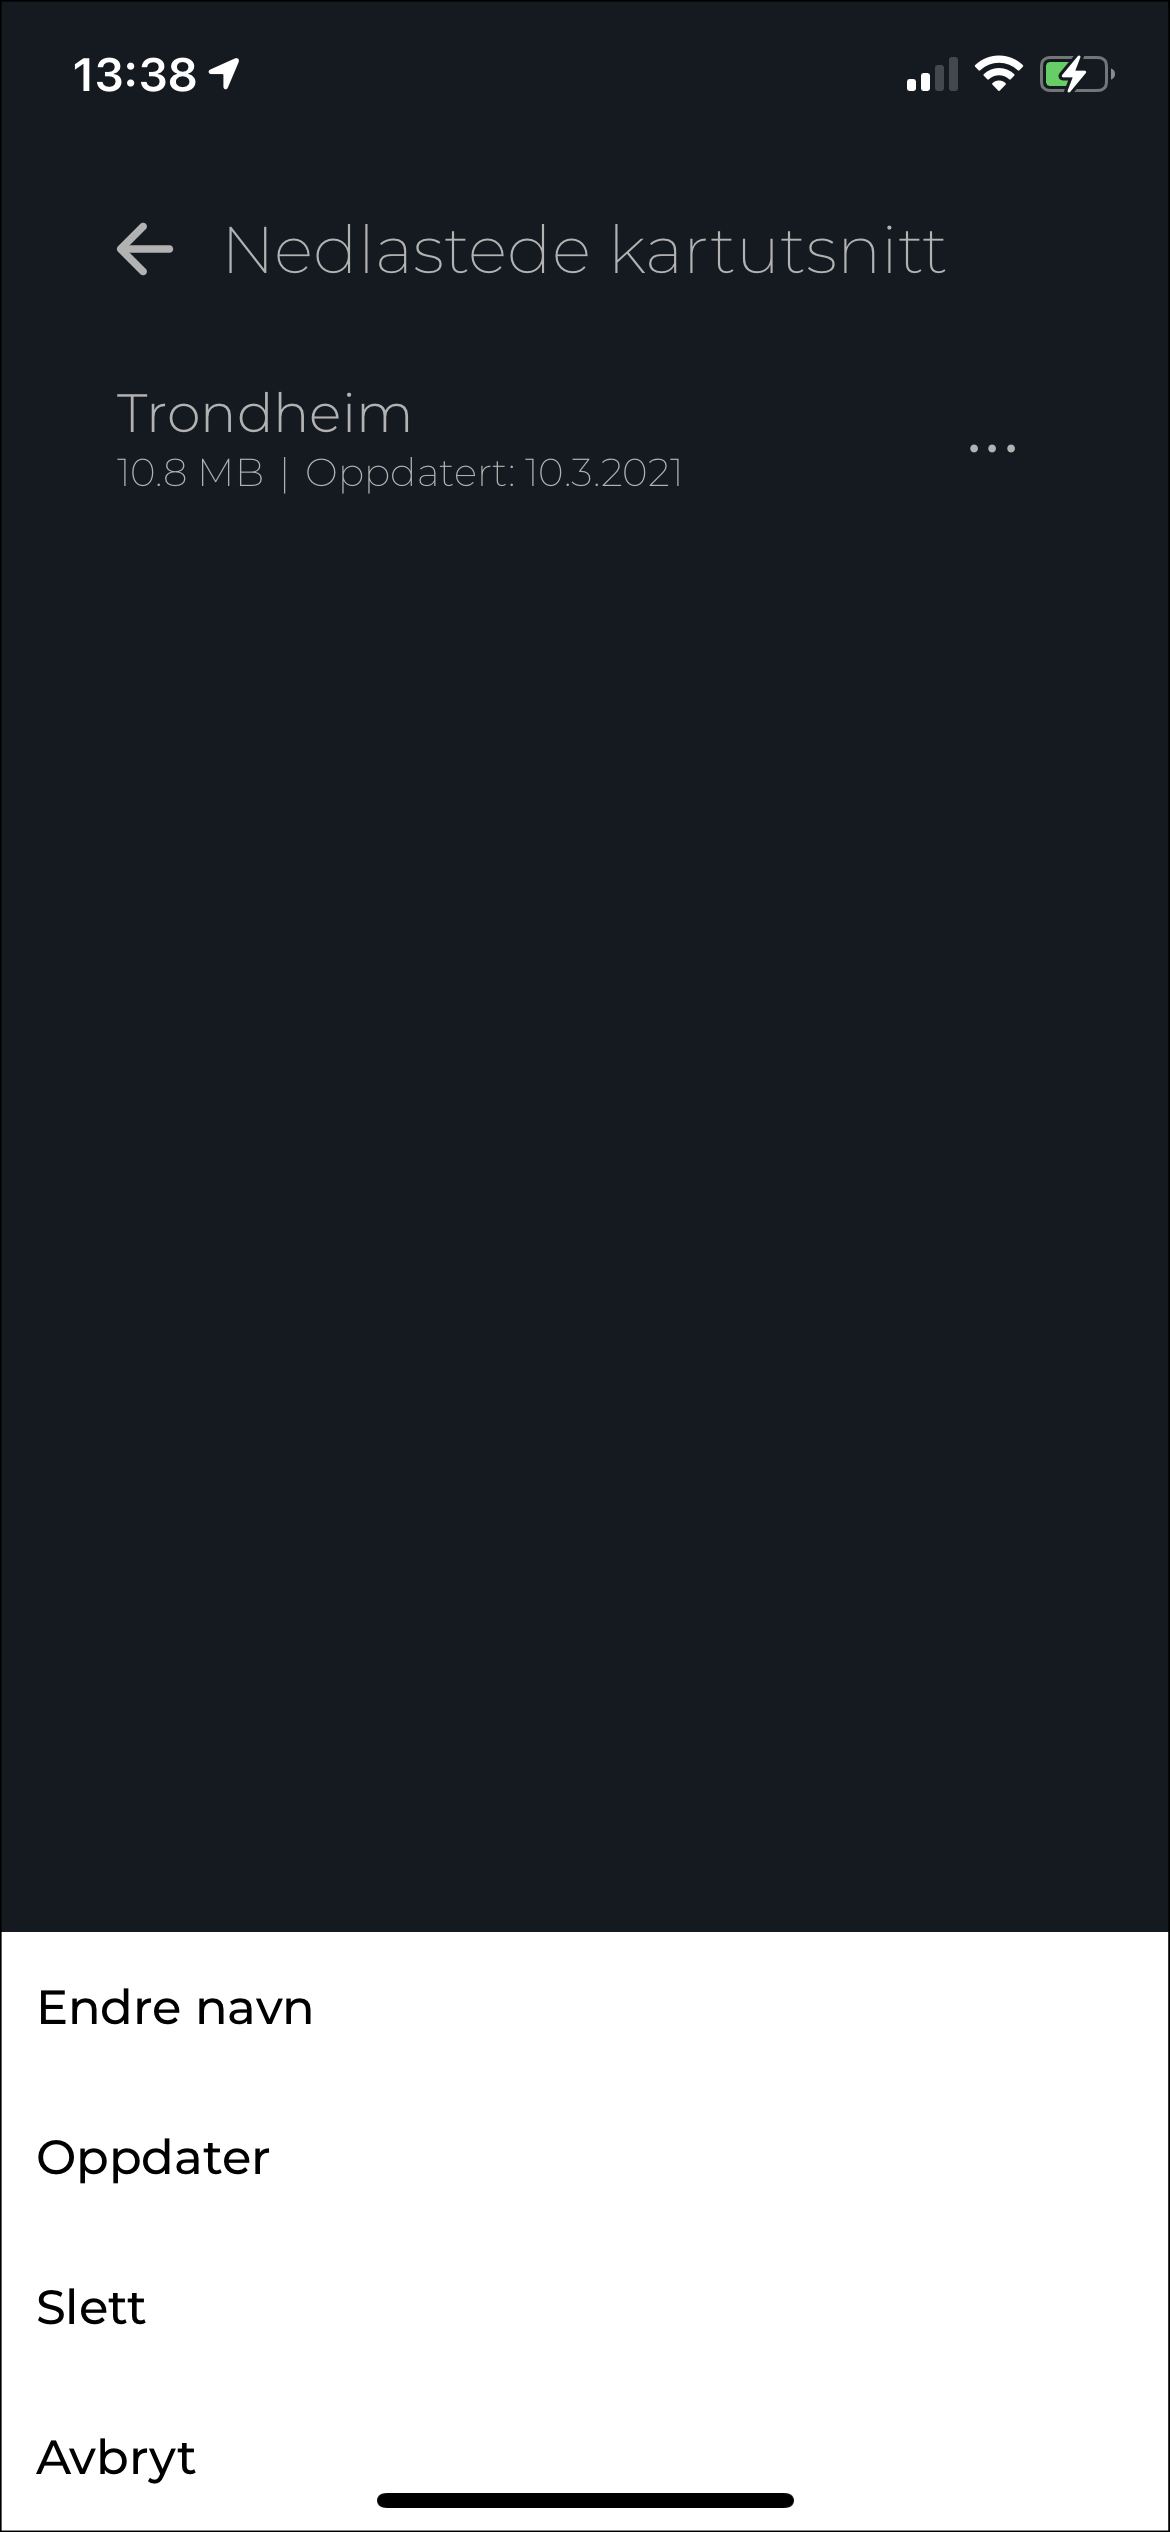
\includegraphics[scale=0.4]{Figurer/skjermbilder/nedlastede-kartutsnitt-apen-meny.png}
    \caption{Valg-meny åpen for et nedlastet kartutsnitt.}
    \label{fig:nedlastede-kartutsnitt-apen-meny}
  \end{minipage}
\end{figure}

\subsubsection{Laste ned nytt kartutsnitt}
For å laste ned et nytt kartutsnitt trykker man på den grønne pluss-knappen vist i figur \ref{fig:nedlastede-kartutsnitt}. Figur \ref{fig:last-ned-nytt-kartutsnitt} viser grensesnittet hvor man velger hvor kartutsnittet skal tas fra og hvor stort det skal være. Her velger man kartutsnittet ved å dra kartet slik at området man ønsker skal komme med havner innenfor det markerte området. Man kan zoome inn og ut for å minske eller øke arealet som det skal lages kartutsnitt av. Grensesnittet er laget helt i henhold til design-prototypen med unntak av pilen for navigering tilbake til siden for nedlastede kartutsnitt. Når man trykker på "Last ned"-knappen starter nedlastingen og man blir tatt tilbake til siden med nedlastede kartutsnitt. Progresjon for nedlastingen vises i grensesnittet i form av en loading-bar som fylles opp til toppen etterhvert som nedlastingen blir ferdig. Når nedlastingen er ferdig vil grensesnittet vise størrelsen på nedlastingen og dato den ble lastet ned. Dette var funksjonalitet som ble designet og implementert etter intern testing da det viste seg at det var behov for en visuell indikator på at kartutsnittet lastes og progresjonen for nedlastingen.
\begin{figure}[H]
  \centering
  \begin{minipage}[b]{0.4\textwidth}
    \centering
    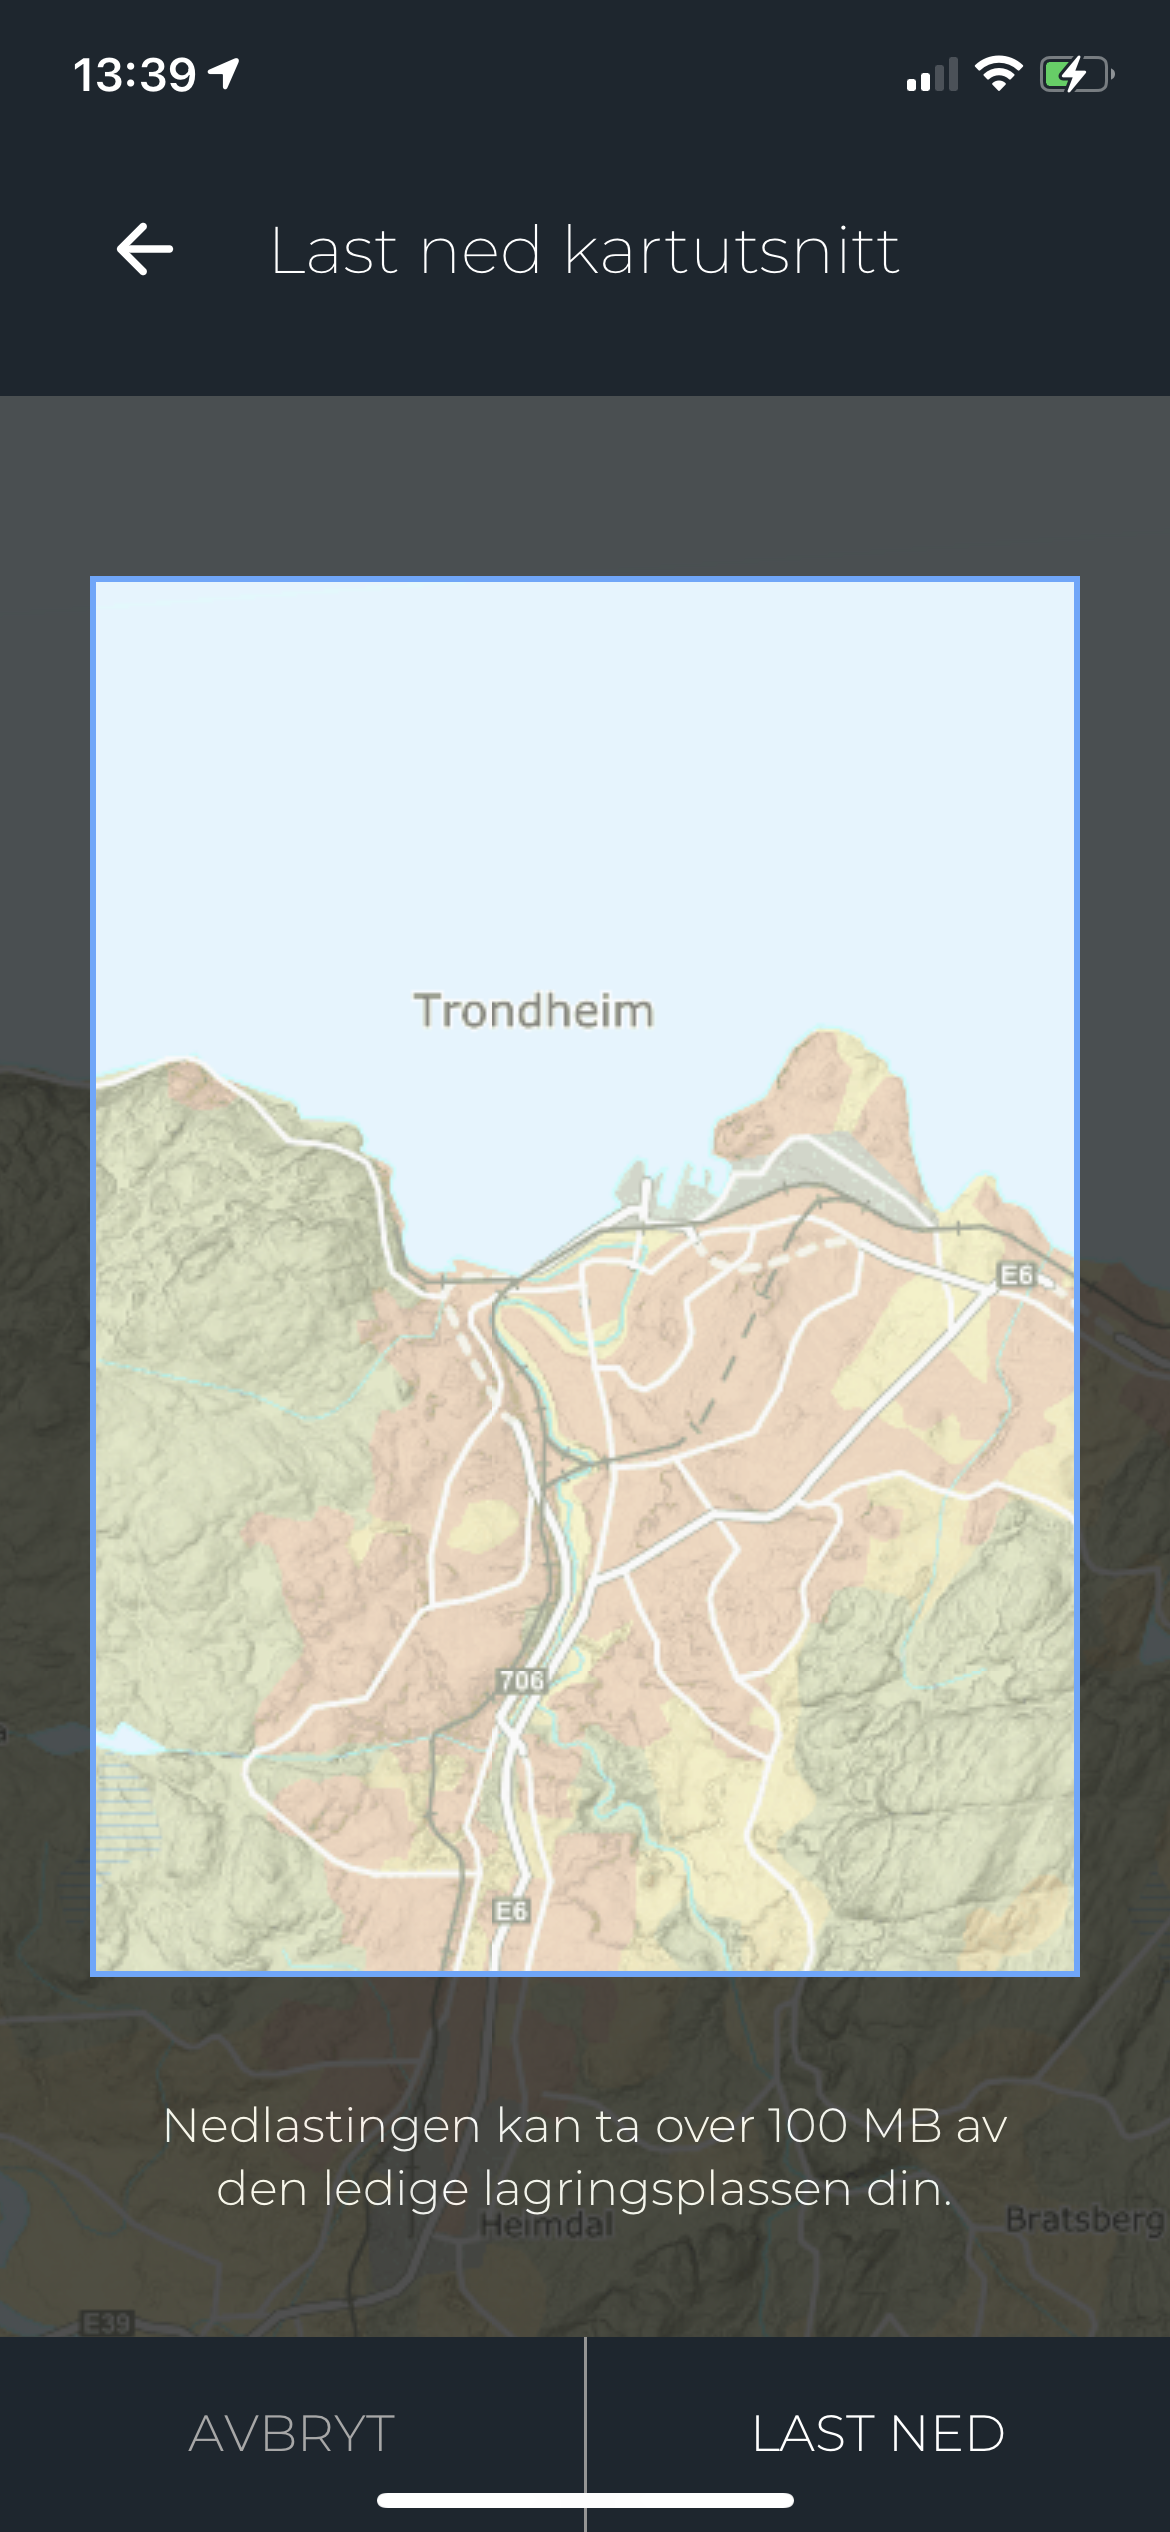
\includegraphics[scale=0.4]{Figurer/skjermbilder/last-ned-nytt-kartutsnitt.png}
    \caption{Side for å laste ned et valg kartutsnitt.}
    \label{fig:last-ned-nytt-kartutsnitt}
  \end{minipage}
  \hfill
  \begin{minipage}[b]{0.4\textwidth}
    \centering
    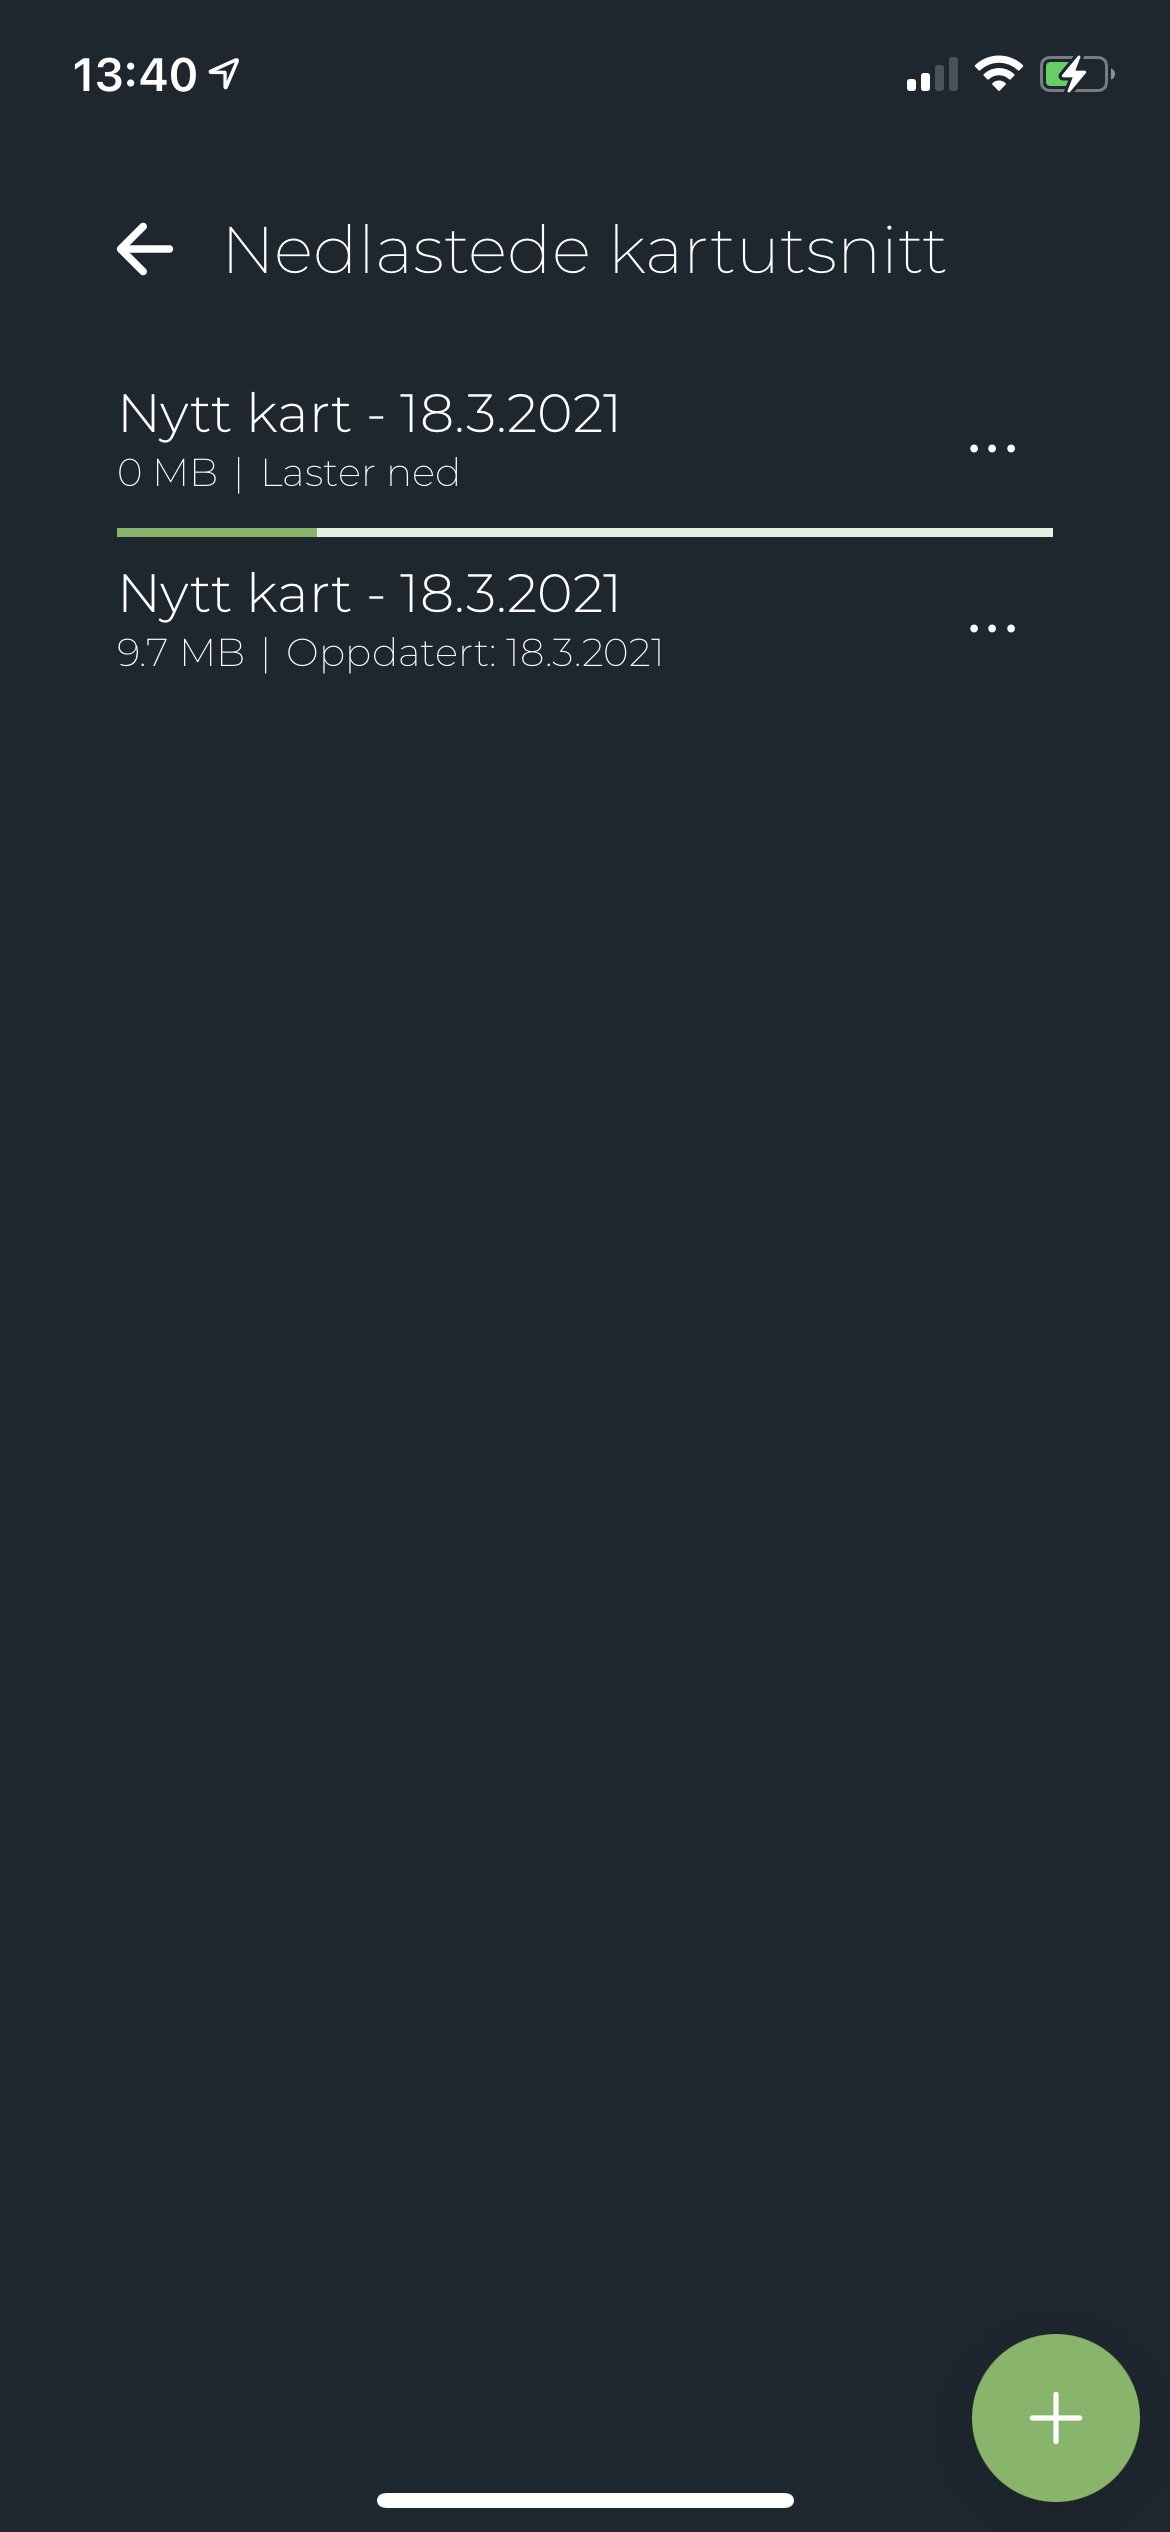
\includegraphics[scale=0.4]{Figurer/skjermbilder/nedlasting-av-nytt-kartutsnitt.png}
    \caption{Progresjon for nedlasting av nytt kartutsnitt.}
    \label{fig:nedlasting-av-nytt-kartutsnitt}
  \end{minipage}
\end{figure}

\noindent
For å laste ned et kartutsnitt brukes cache-tjenesten til Geonorge i form av \textit{opencache}-endepunktene. Cache-tjenestene bygger på underliggende \acrshort{wms}-tjenester, noe som gjør dem svært brukbare i webapplikasjoner \cite{GeoNorgeLeaflet}. Kartet er lagret på tjeneren i form av fliser. Med dette menes det at kartet er delt inn i rektangulære bilder med ulikt detaljnivå basert på hvor zoomet inn man er. For å få tak i en bestemt flis må man oppgi x- og y-koordinaten til flisen, samt zoom-nivå. Et eksempel på et kall til tjenesten er:
\url{https://opencache.statkart.no/gatekeeper/gk/gk.open_gmaps?layers=norges_grunnkart&zoom=14&x=8665&y=4429}. Her hentes flisen med x-koordinat 8665, y-koordinat 4429 og zoom-nivå 14 ut fra tjeneren.
\begin{figure}[H]
\centering
\captionsetup{width=.8\linewidth}
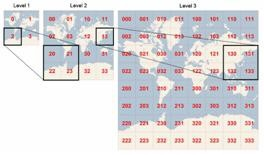
\includegraphics[scale=1.0]{Figurer/Bilder/tilesitiles.jpg}
\caption{Illustrasjon av hvordan kartet er delt inn i fliser.}
\label{fig:map-tiles}
\source{\cite{GeoNorgeLeaflet}}
\end{figure}

\noindent
For at kartet skal fungere uten internett må hver eneste flis for det valgte kartutsnittet lastes ned og lagres på en måte som gjør det mulig å hente ut en bestemt flis basert på x- og y-koordinat og zoom-nivå. Denne prosessen starter med at piksel-koordinatene for øvre venstre hjørne og nedre høyre hjørne for rektangelet som markerer kartutsnittet (se figur \ref{fig:figma-laste-ned-kartutsnitt}) gjøres om det GPS-koordinater. Det kan enkelt gjøres med en innbygd metode i Leaflet kalt containerPointToLatLng({x, y}) \cite{LeafletDom}. Deretter kan GPS-koordinater gjøres om til flis-koordinater med en standardisert metode \cite{SlippyMapTilenames}. Under nedlastingen sendes forespørsler til Cache-tjenesten for å laste ned alle kart-flisene fra øvre venstre til nedre høyre hjørne, for hvert spesifiserte zoom-nivå. For å balansere lasten på tjeneren veksles det mellom å bruke endepunktene opencache.statkart.no, opencache2.statkart.no og opencache3.statkart.no.
\newline

\noindent
For at Lealet skal klare å hente ut korrekt kart-flis fra det lokale filsystemet på mobiltelefonen, må kartflisene lagres på en måte som gir en URI lik den som benyttes når kart-flisene hentes direkte fra tjeneren. Figur \ref{fig:kartutsnitt-lagring} viser hvordan denne filstrukturen er delt opp. For å hente ut kart-flisen spesifisert i figuren bruker Leaflet URI-en \url{maps/421-A3-AD1/mapTiles/14/8665/4429/mapTile.b64}. En metadata-fil lagres også sammen med kart-flisene med informasjon som tilhører det nedlastede kartutsnittet. Metadata som lagres om kartet er kartutsnittets navn, størrelse (i bytes), nedlastingsdato og lokasjon. Denne metadata-filen brukes for å vise fram nyttig informasjon til brukeren, men også for å utføre intern logikk i programmet som for eksempel når et kart skal oppdateres.  

\begin{figure}[H]
\centering
\captionsetup{width=.8\linewidth}
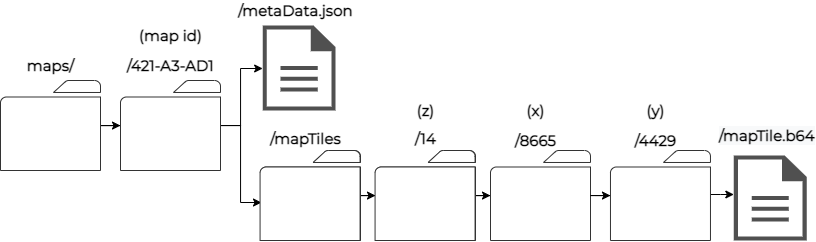
\includegraphics[scale=0.5]{Figurer/diagram/kartutsnitt-lagring.png}
\caption{Eksempel på lagringsstruktur for kartutsnitt med id 423-A3-AD1 og tilhørende kart-flis med koordinater z = 14, x = 8665 og y = 4429.}
\label{fig:kartutsnitt-lagring}
\end{figure}

\subsection{Ny oppsynstur}
\subsubsection{Registrering av informasjon for ny oppsynstur.}
Grensesnittet for registrering av informasjon i sammenheng med en ny oppsynstur har blitt implementert i henhold til design-prototypen. Navnet til brukeren som allerede er logget inn legges til automatisk i listen over deltagere.
\begin{figure}[H]
\centering
\captionsetup{width=.8\linewidth}
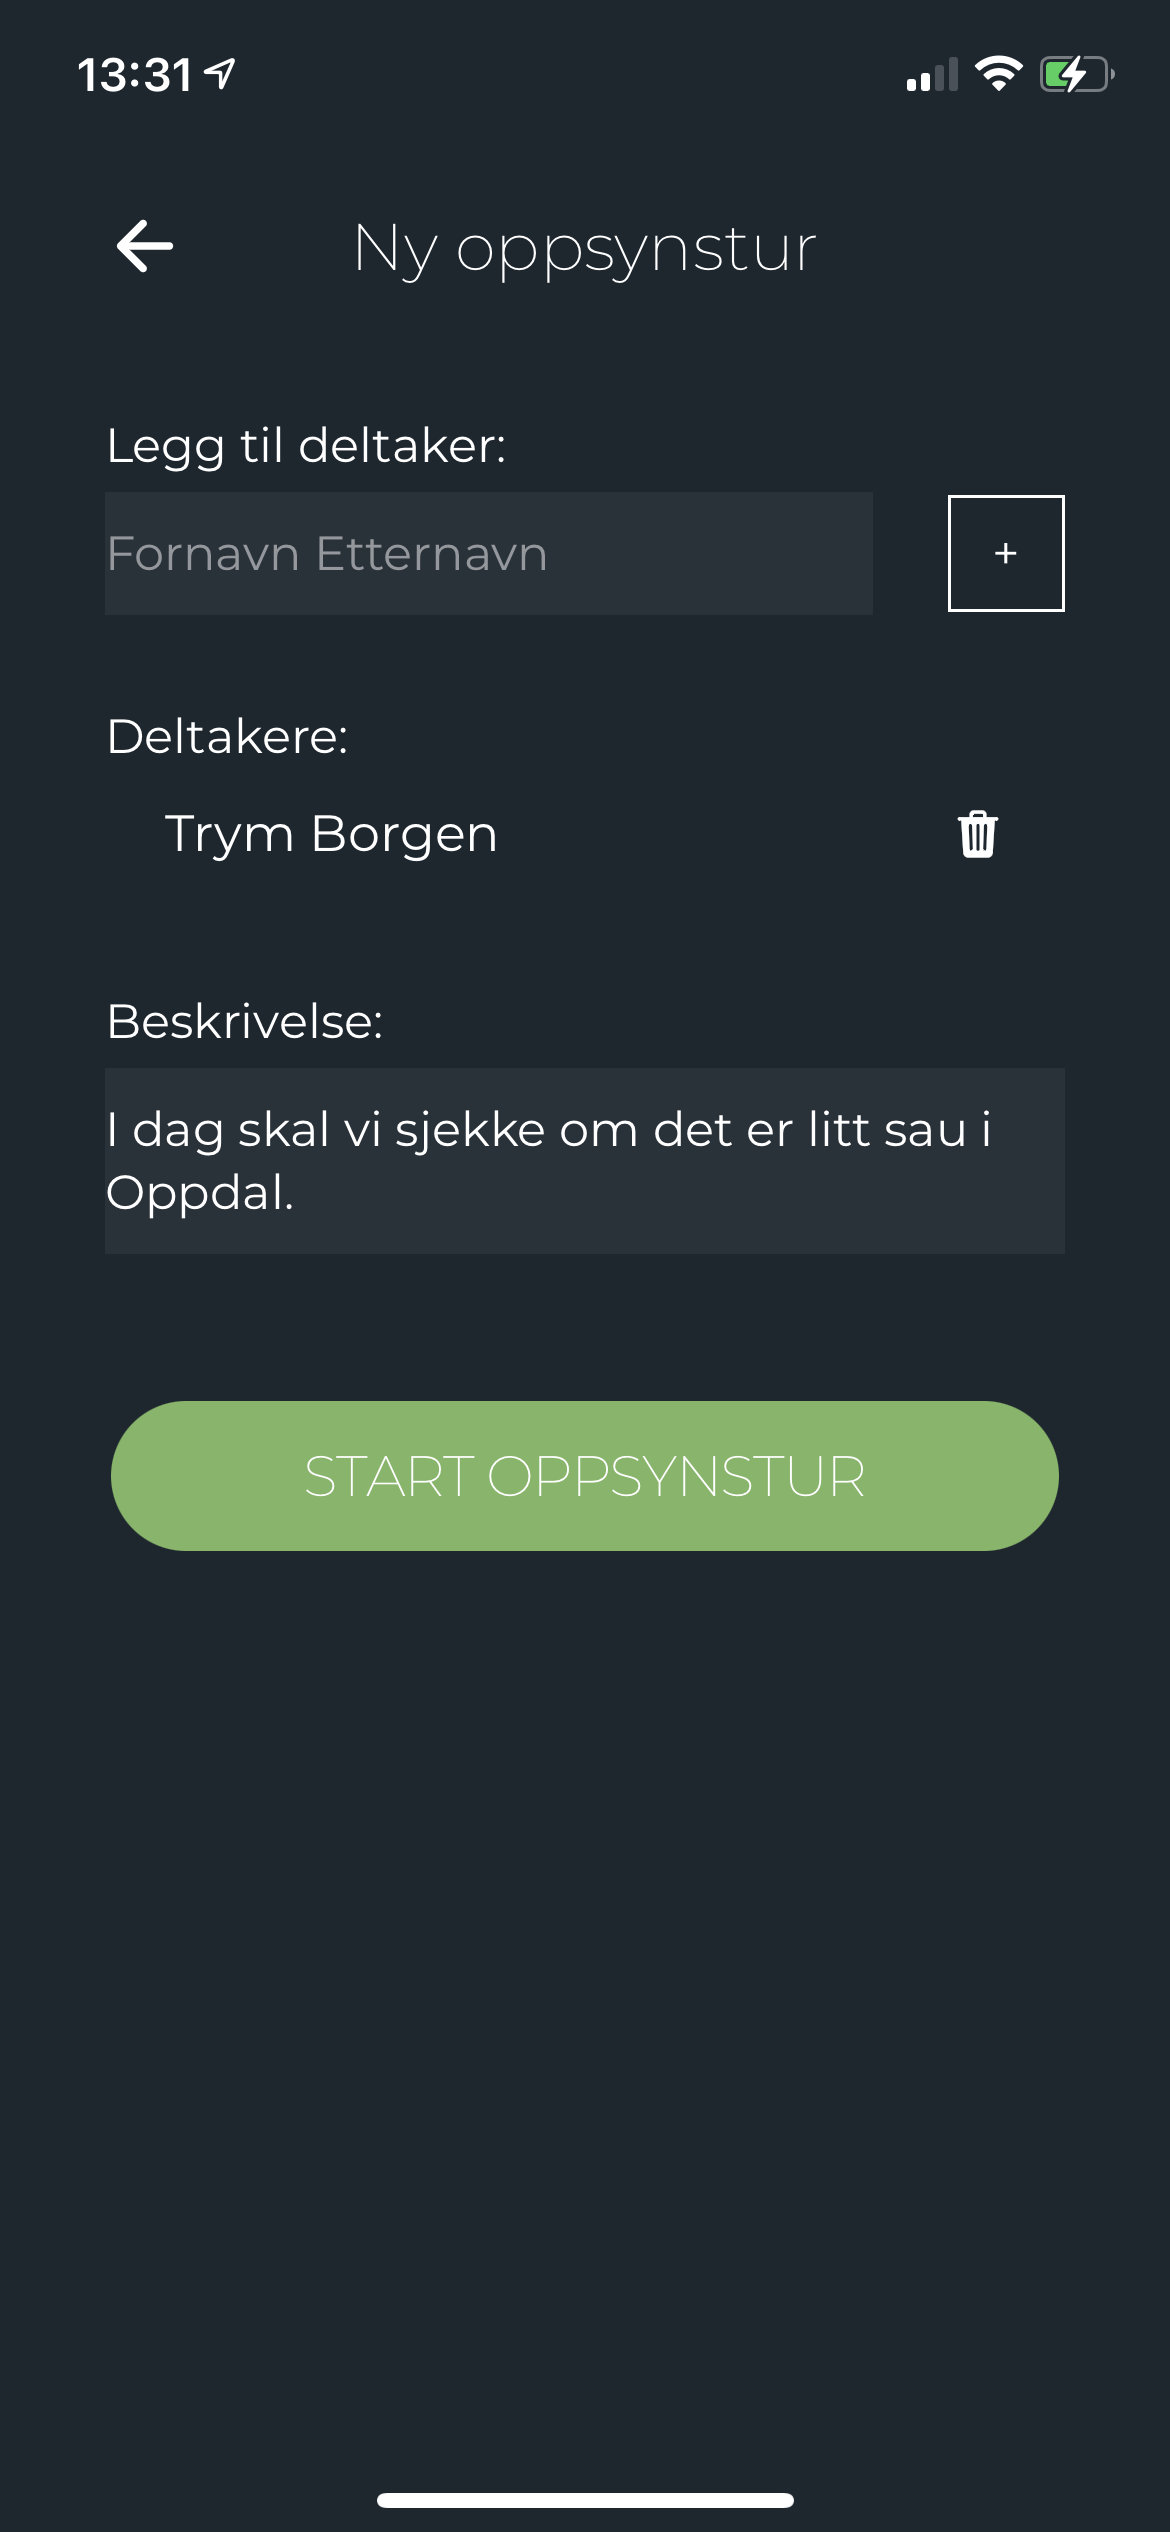
\includegraphics[scale=0.4]{Figurer/skjermbilder/info-oppsynstur.png}
\caption{Implementert grensesnitt for registrering av informasjon før ny oppsynstur.}
\label{fig:info-oppsysntur}
\end{figure}

\subsubsection{Kart}
Kartgrensesnittet som brukes under en en oppsynstur har blitt implementert i henhold til design-prototypen med visse endringer. For det første har størrelsen på symbolene blitt redusert for å gi mer plass til selve kartet. Markøren som viser hvor en registrering blir plassert, som vist i midten av kartet på figur \ref{fig:kart-meny-apen}, har blitt byttet ut med en tydeligere markør som gjør det mulig se sentrum av hva man registrer. Det har også blitt lagt til en knapp nederst i midten av grensesnittet. Denne knappen kan brukes til å sette applikasjonen i strømsparingsmodus som forklares nærmere i underkapittel \ref{sec:bakgrunnsoppdatering-av-gps-lokasjon} \nameref{sec:bakgrunnsoppdatering-av-gps-lokasjon}.

\begin{figure}[H]
  \centering
  \begin{minipage}[b]{0.4\textwidth}
    \centering
    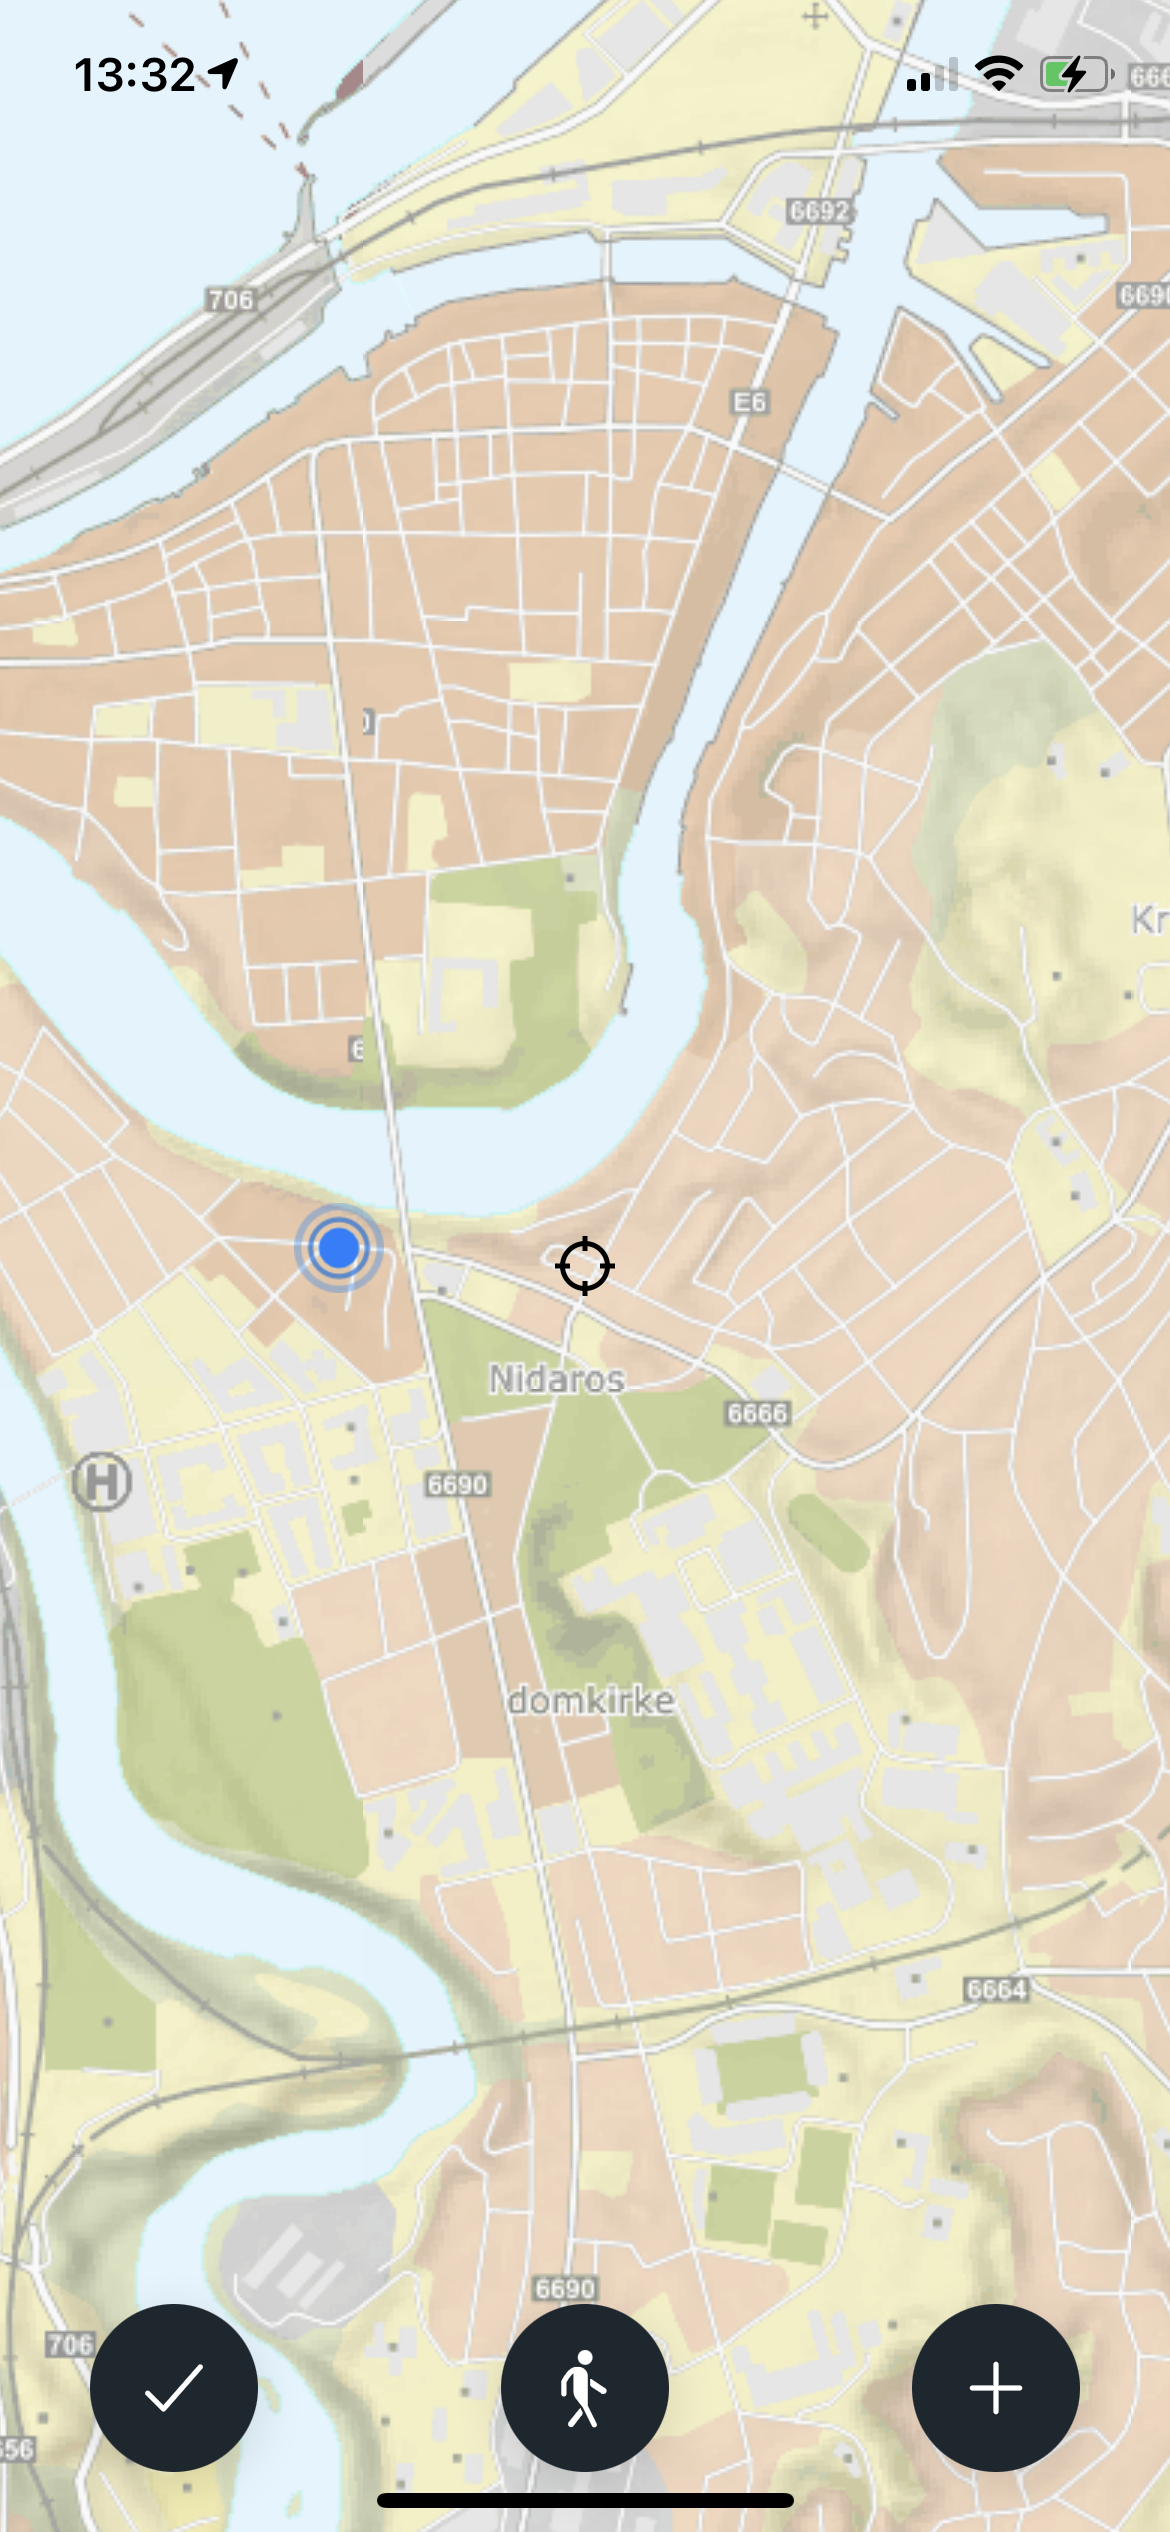
\includegraphics[scale=0.4]{Figurer/skjermbilder/kart-plain.png}
    \caption{Implementert grensesnitt for interaksjon med kart under registrering.}
    \label{fig:kart-plain}
  \end{minipage}
  \hfill
  \begin{minipage}[b]{0.4\textwidth}
    \centering
    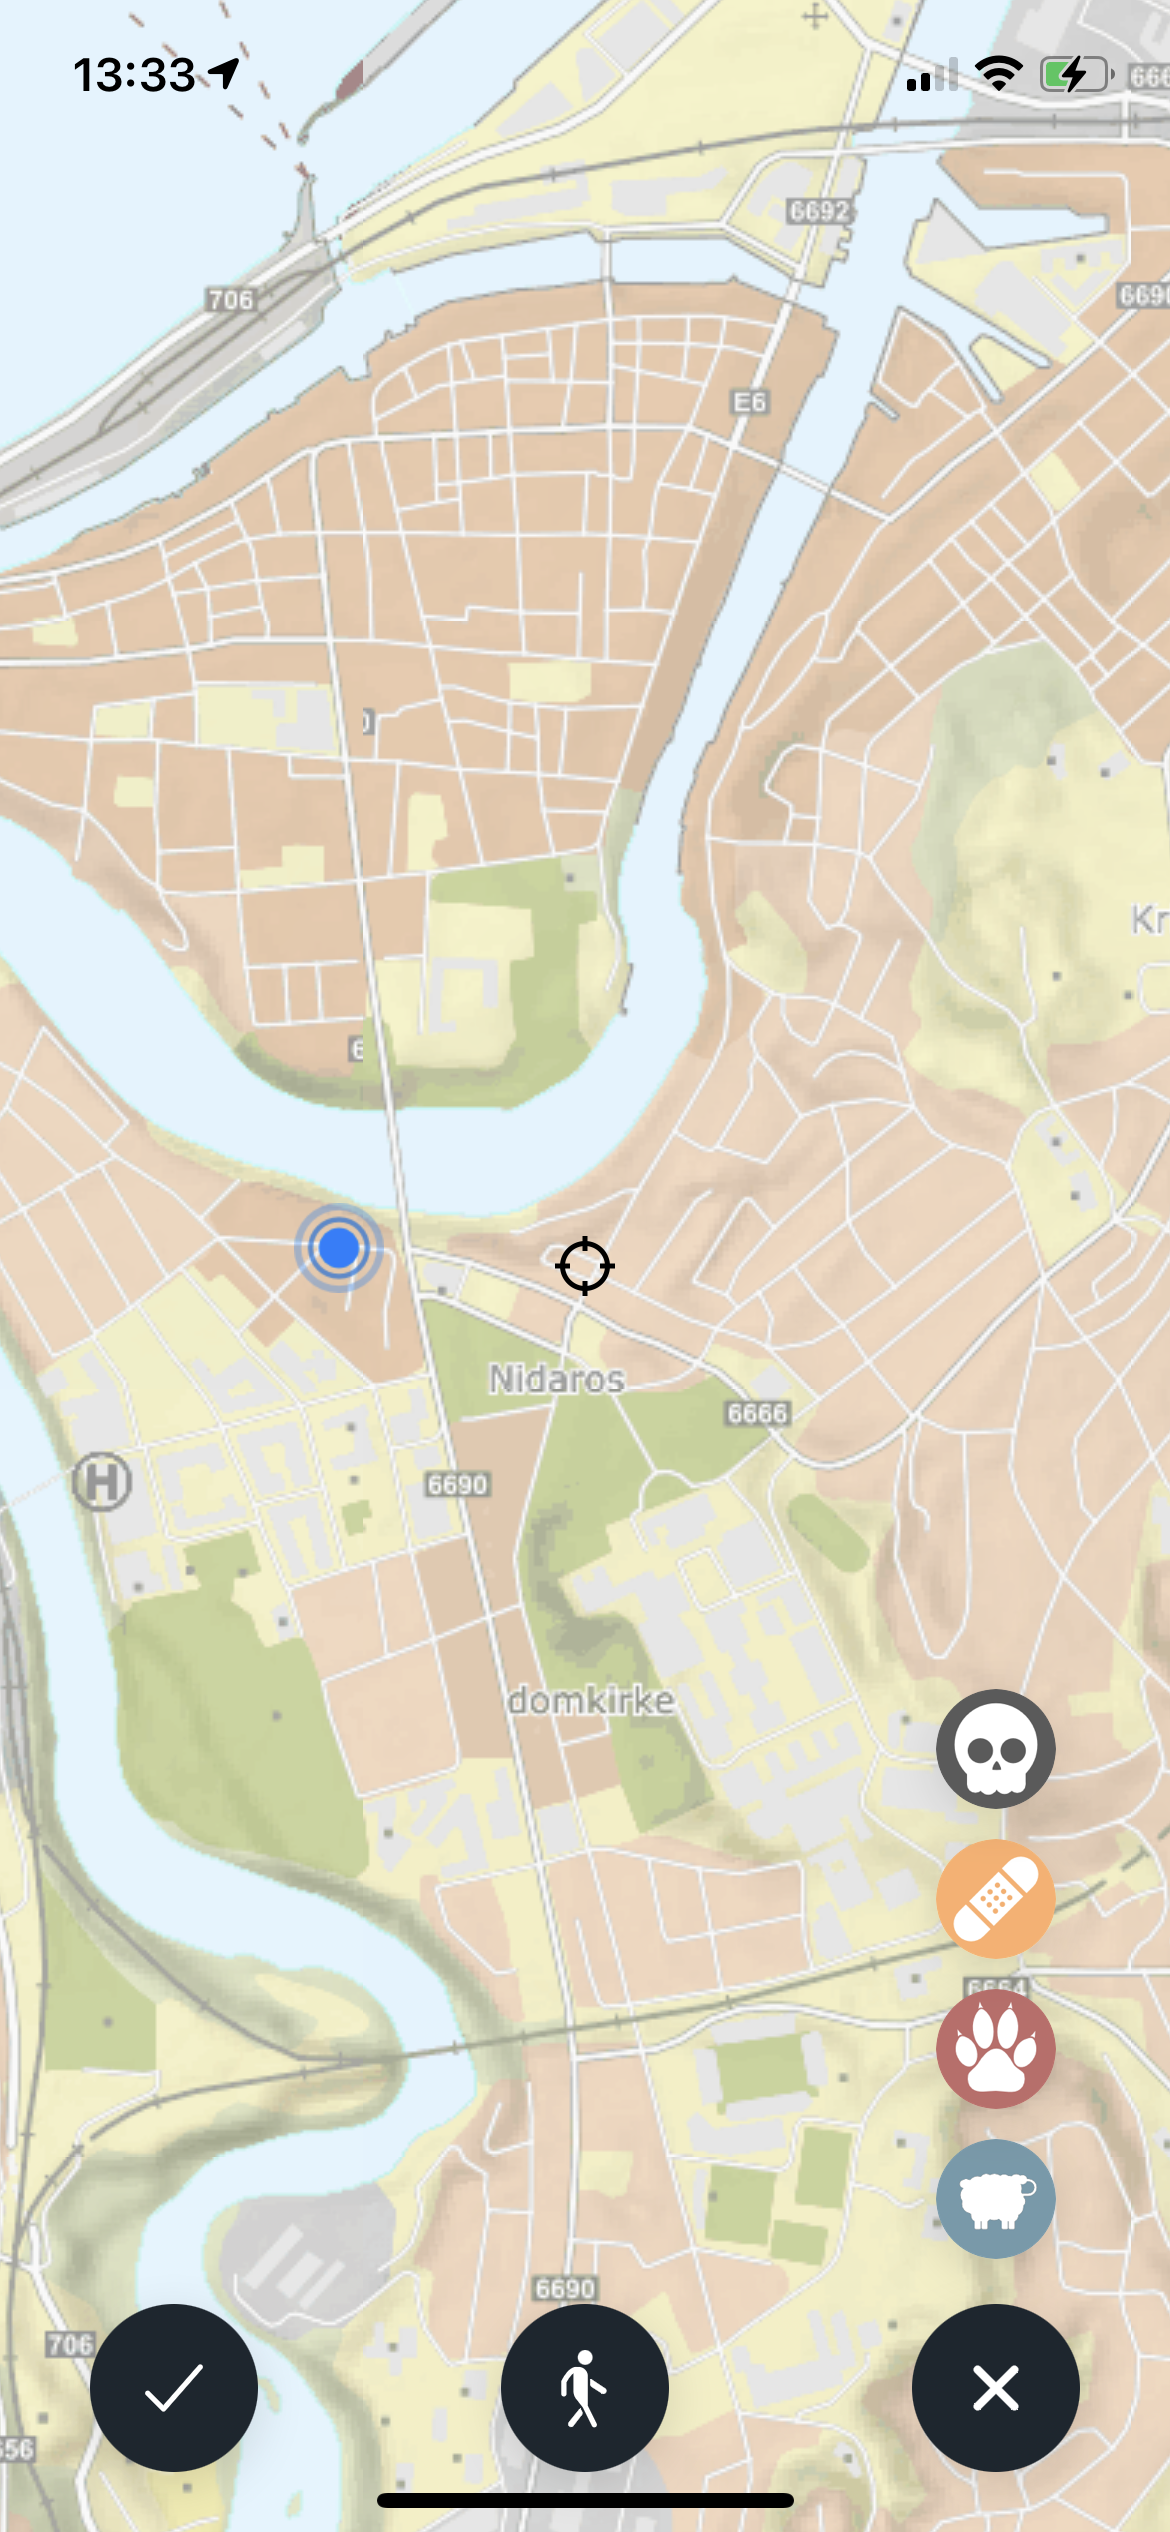
\includegraphics[scale=0.4]{Figurer/skjermbilder/kart-meny-apen.png}
    \caption{Kart-grensesnitt med åpen meny for å legge til en ny registrering.}
    \label{fig:kart-meny-apen}
  \end{minipage}
\end{figure}

\noindent
Kartgrensesnittet tar i bruk \textit{Norgeskart bakgrunn cache} \cite{NorgeskartBakgrunnCache} fra Geonorge som er utviklet av Kartverket og brukes sammen med Leaflet-biblioteket \cite{LeafletJavaScriptLibrary} for å vise fram kartet. Kartet oppdateres daglig slik at gjetere og bønder alltid vil ha tilgang til de nyeste kartbildene under en oppsynstur. Den blå markøren på kartet viser GPS-posisjonen til brukeren av applikasjonen. Markørens posisjon oppdateres i sanntid. Man kan navigere kartet ved å dra det rundt med bruk av én finger. "Pinch-zoom"-funksjonalitet er innebygd i Leaflet \cite{ZoomLevelsLeaflet} og tillater å zoome inn og ut ved hjelp av to fingre. Hvis mobiltelefonen ikke er koblet til internett vil applikasjonen automatisk velge det nedlastede kartutsnittet som passer best for den nåværende lokasjonen til mobiltelefonen. Hvis ingen nedlastede kartutsnitt passer vil brukeren få tilbakemelding om dette. Applikasjonen har også implementert funksjonalitet for å skifte mellom ulike nedlastede kartutsnitt hvis dette er nødvendig.
\newline

\noindent
For legge til en ny registrering i kartet kan brukeren trykke på pluss-knappen nede i høyre hjørne av skjermen. Dette vil åpne valg-menyen (se figur \ref{fig:kart-meny-apen}) for en ny registrering der brukeren kan velge mellom å registrere en saueflokk, et rovdyr, skadede sau eller døde sau. Menyen kan lukkes ved å trykke på den samme knappen om igjen, markert ved at pluss-tegnet har blitt byttet ut med et kryss. Registreringsmarkøren i midten av kartet plasseres over den posisjon hvor man har gjort en observasjon. Denne posisjonen brukes sammen med brukerens GPS-lokasjon, og type registrering (sau, død, skadet eller rovdyr) for å kunne legge til registreringen i kartet. Figur \ref{fig:registrert-rovdyr} viser hvordan kartgrensesnittet ser ut rett etter registrering av et rovdyr. En pin blir lagt til på kartet på posisjonen hvor observasjonen ble gjort. En striplet linje peker fra GPS-lokasjoen til brukeren under observasjonstidspunktet og fram til pinnen. Både pinnen og den striplede linjen er fargekodet for å gjøre det lettere å skille mellom ulike observasjoner.

\begin{figure}[H]
\centering
\captionsetup{width=.8\linewidth}
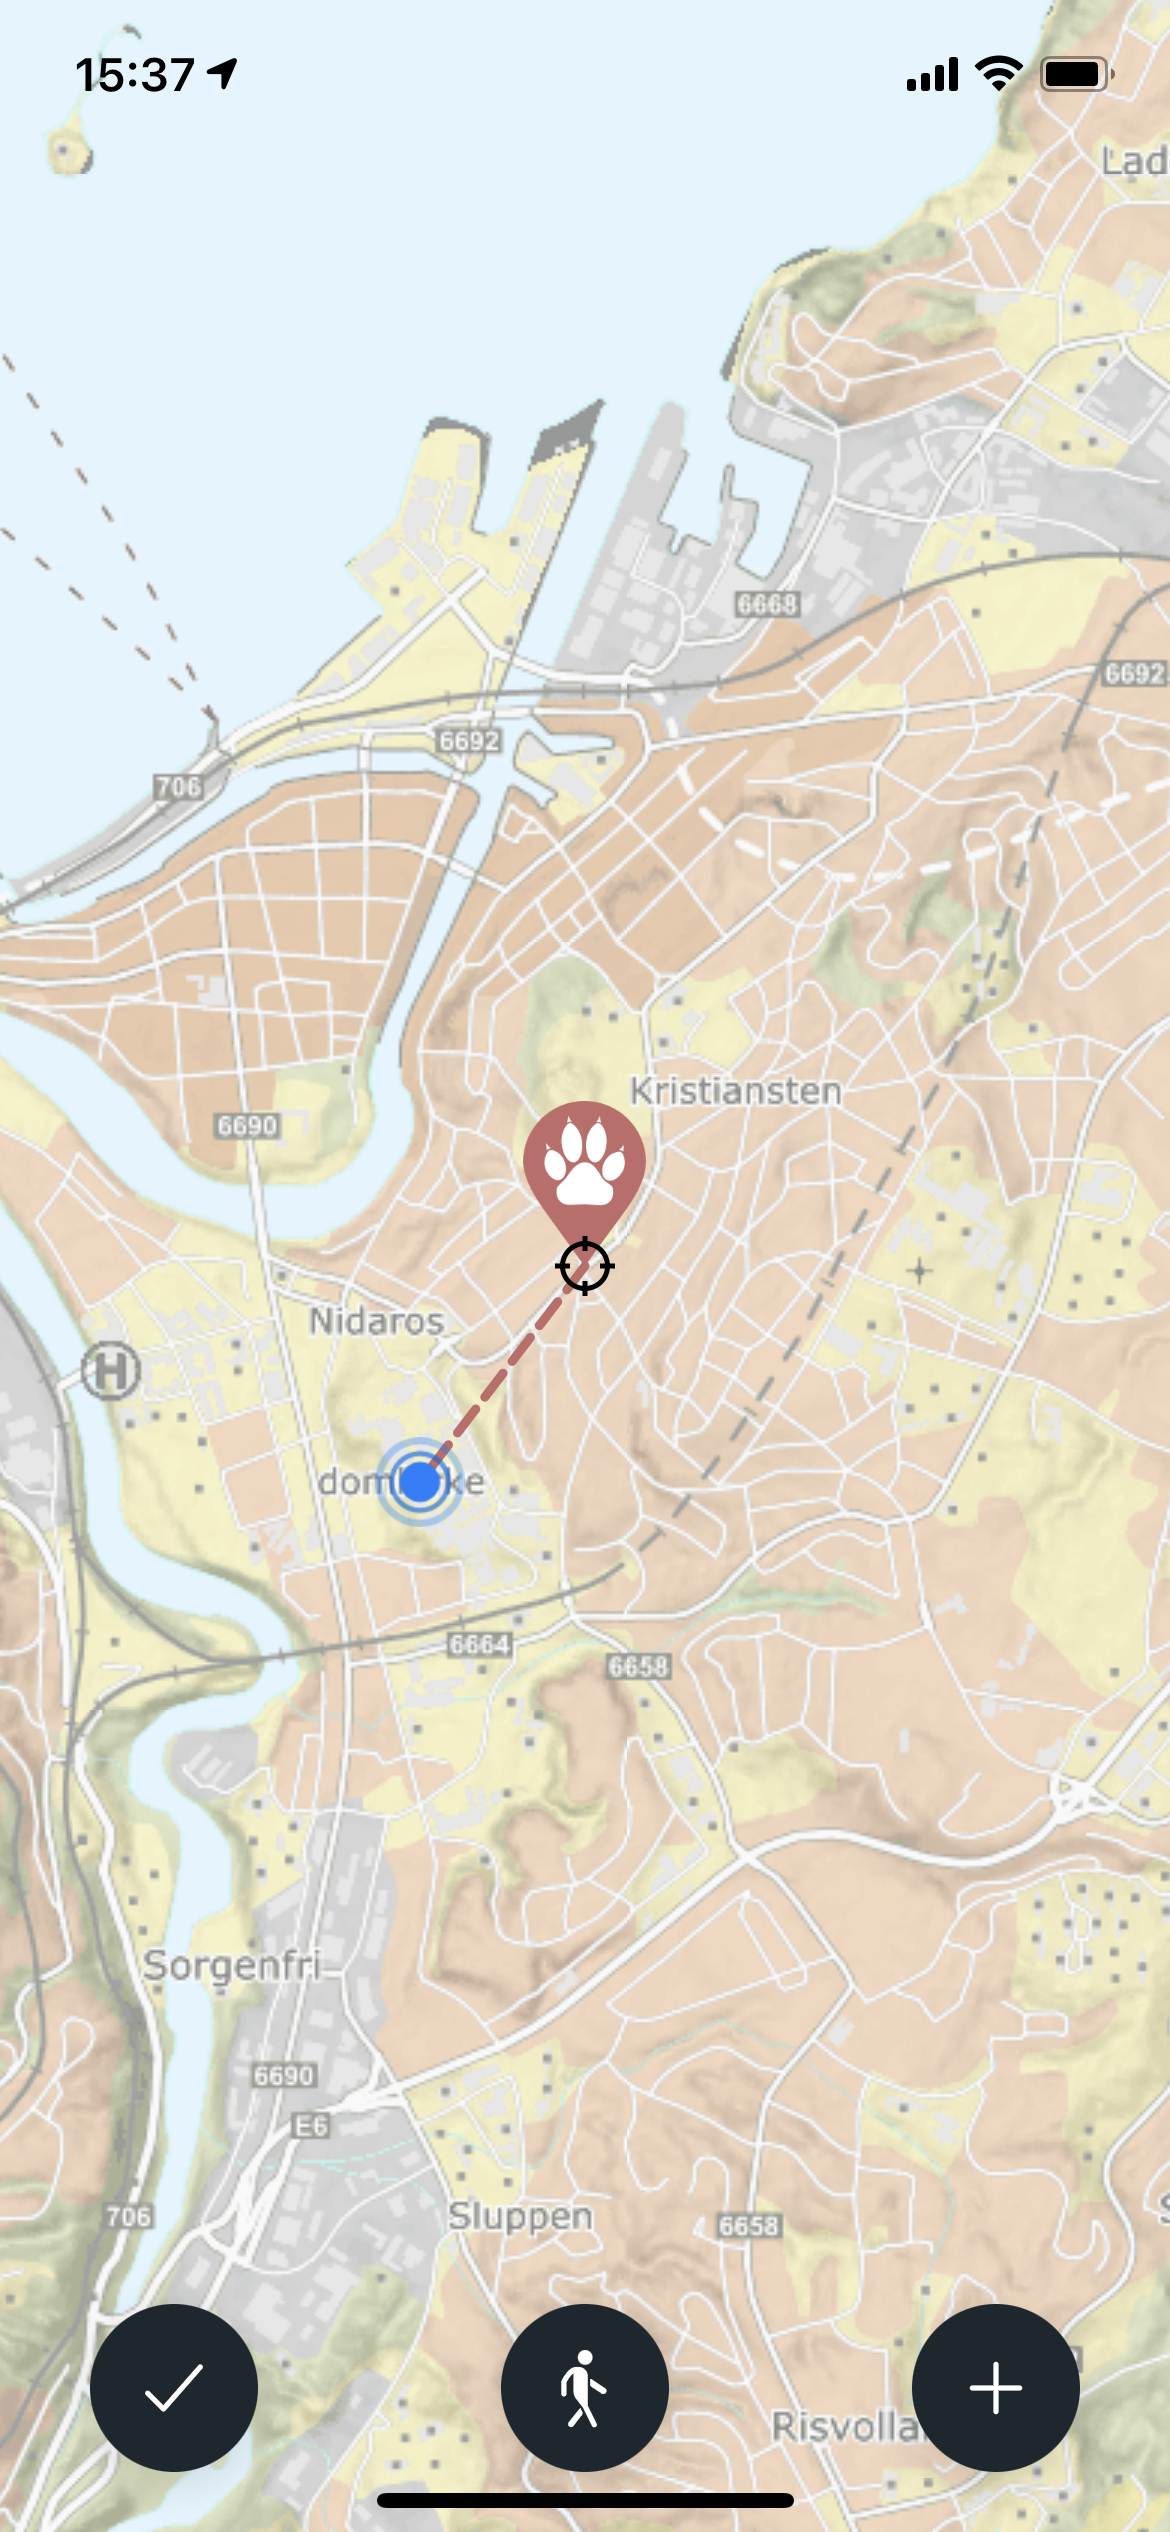
\includegraphics[scale=0.4]{Figurer/skjermbilder/registert-rovdyr.png}
\caption{Eksempel på hvordan kartgrensesnittet ser ut etter at det har blitt registrert et rovdyr.}
\label{fig:registrert-rovdyr}
\end{figure}

\subsubsection{Fullføre oppsyntur}
For å fullføre en oppsynstur trykker brukeren på fullfør-knappen nede til venstre i kartgrensesnittet (se figur \ref{fig:registrert-rovdyr}). En dialogboks, som vist i figur \ref{fig:follfore-oppsynstur}, vil da vises hvor brukeren må bekrefte handlingen. Hvis brukren trykker ja vises oppsummeringssiden fram (se figur \ref{fig:oppsynstur-oppsummering}).

\begin{figure}[H]
  \centering
  \begin{minipage}[b]{0.4\textwidth}
    \centering
    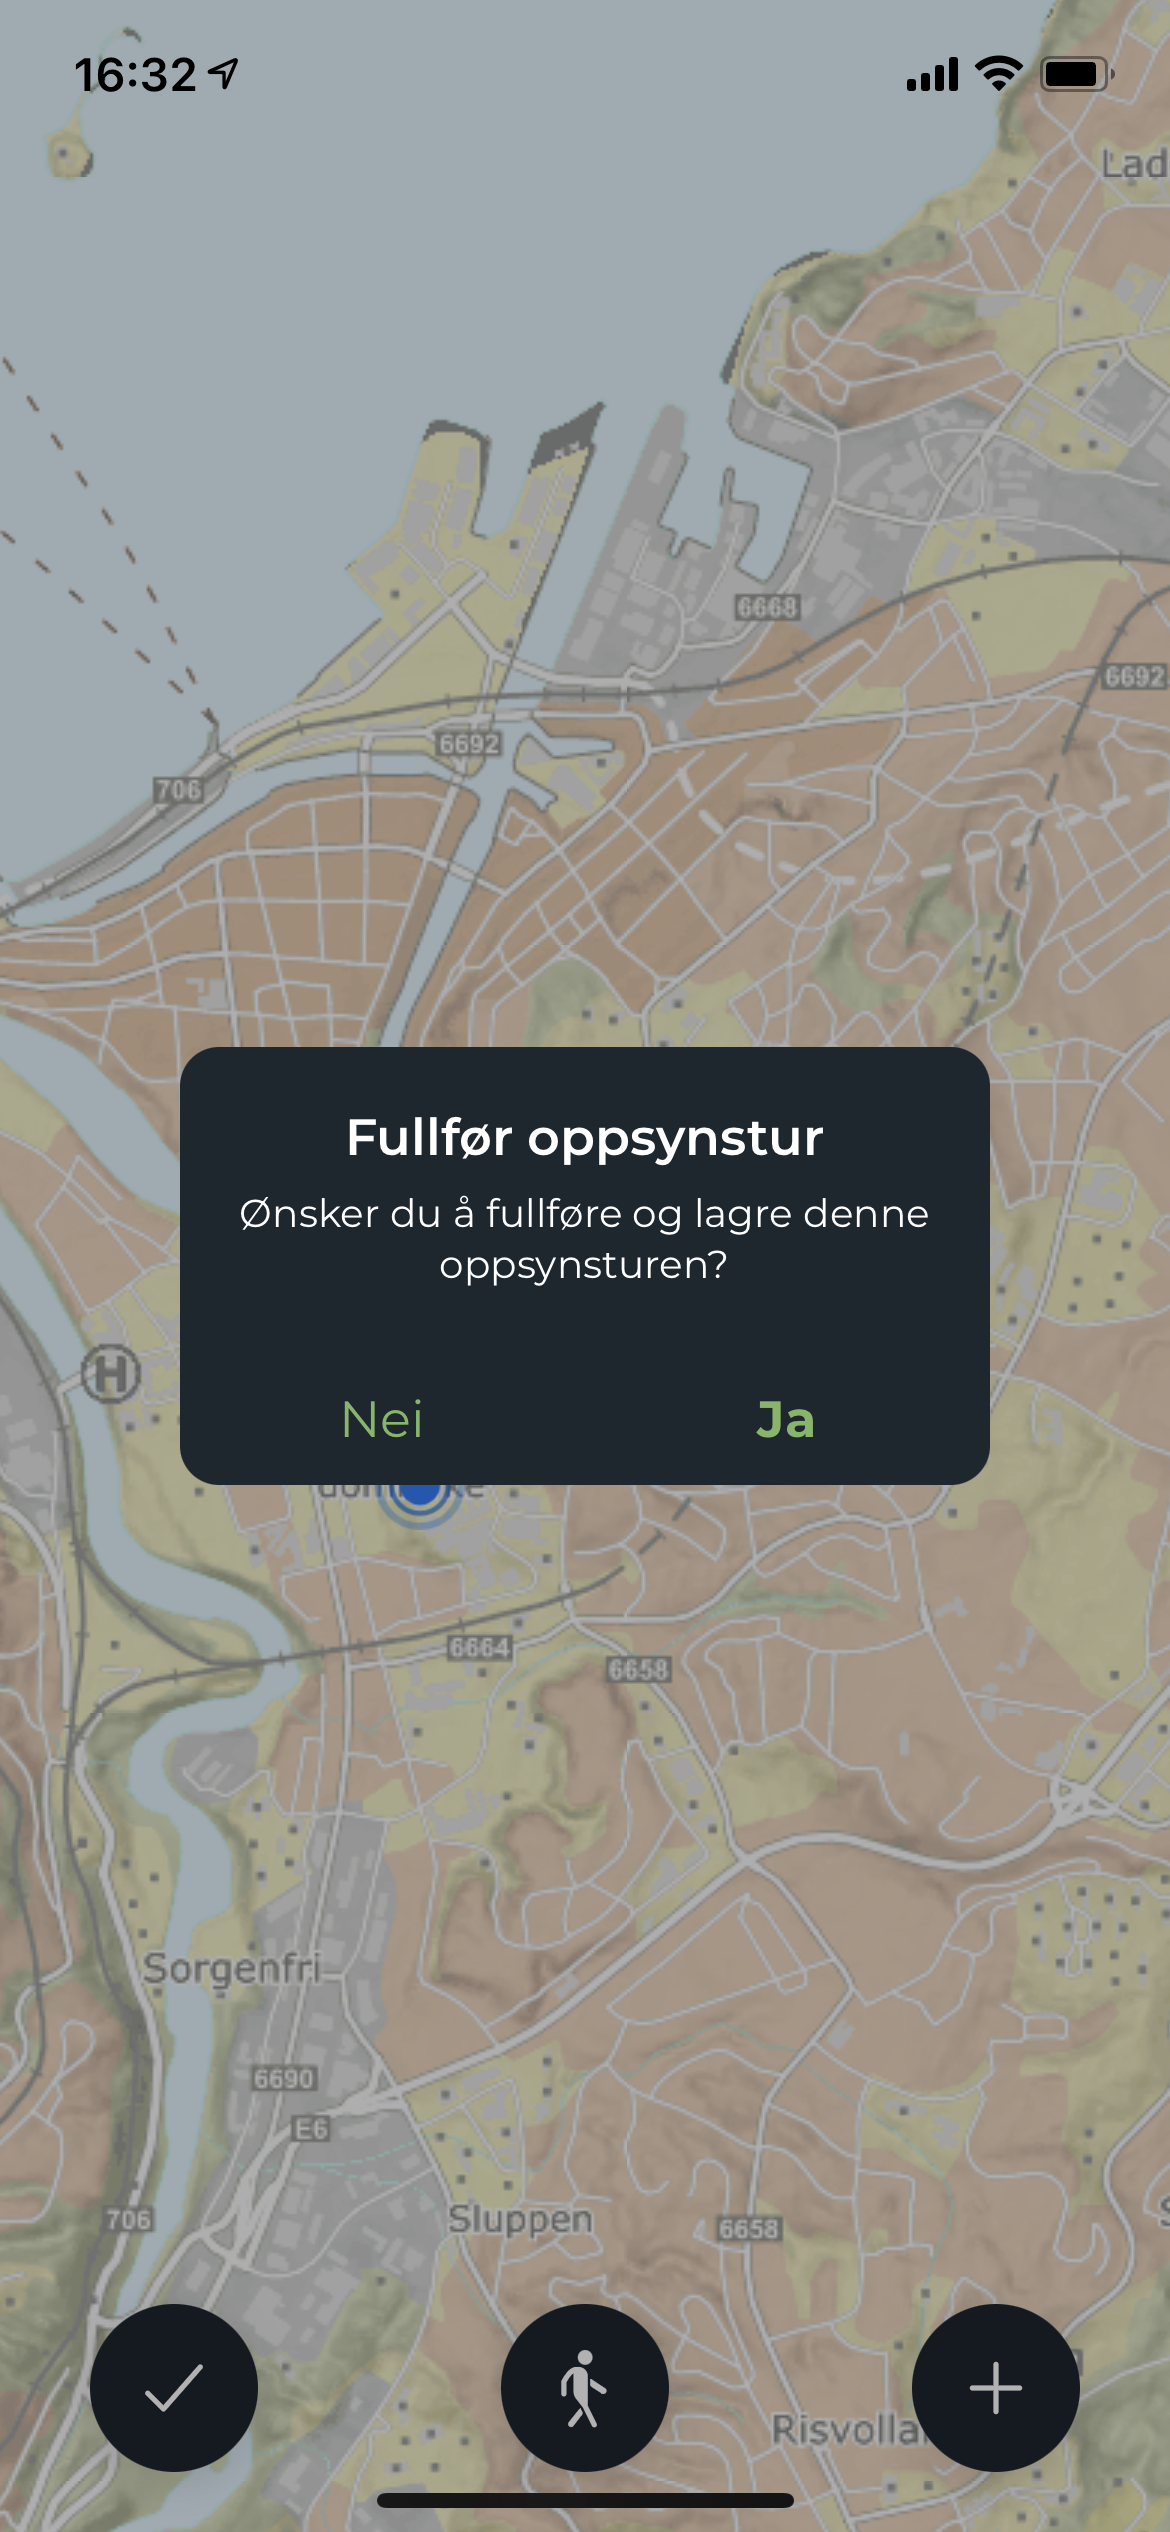
\includegraphics[scale=0.4]{Figurer/skjermbilder/follfore-oppsynstur.png}
    \caption{Dialogboks som kommer opp hvis man trykker på fullfør-knappen.}
    \label{fig:follfore-oppsynstur}
  \end{minipage}
  \hfill
  \begin{minipage}[b]{0.4\textwidth}
    \centering
    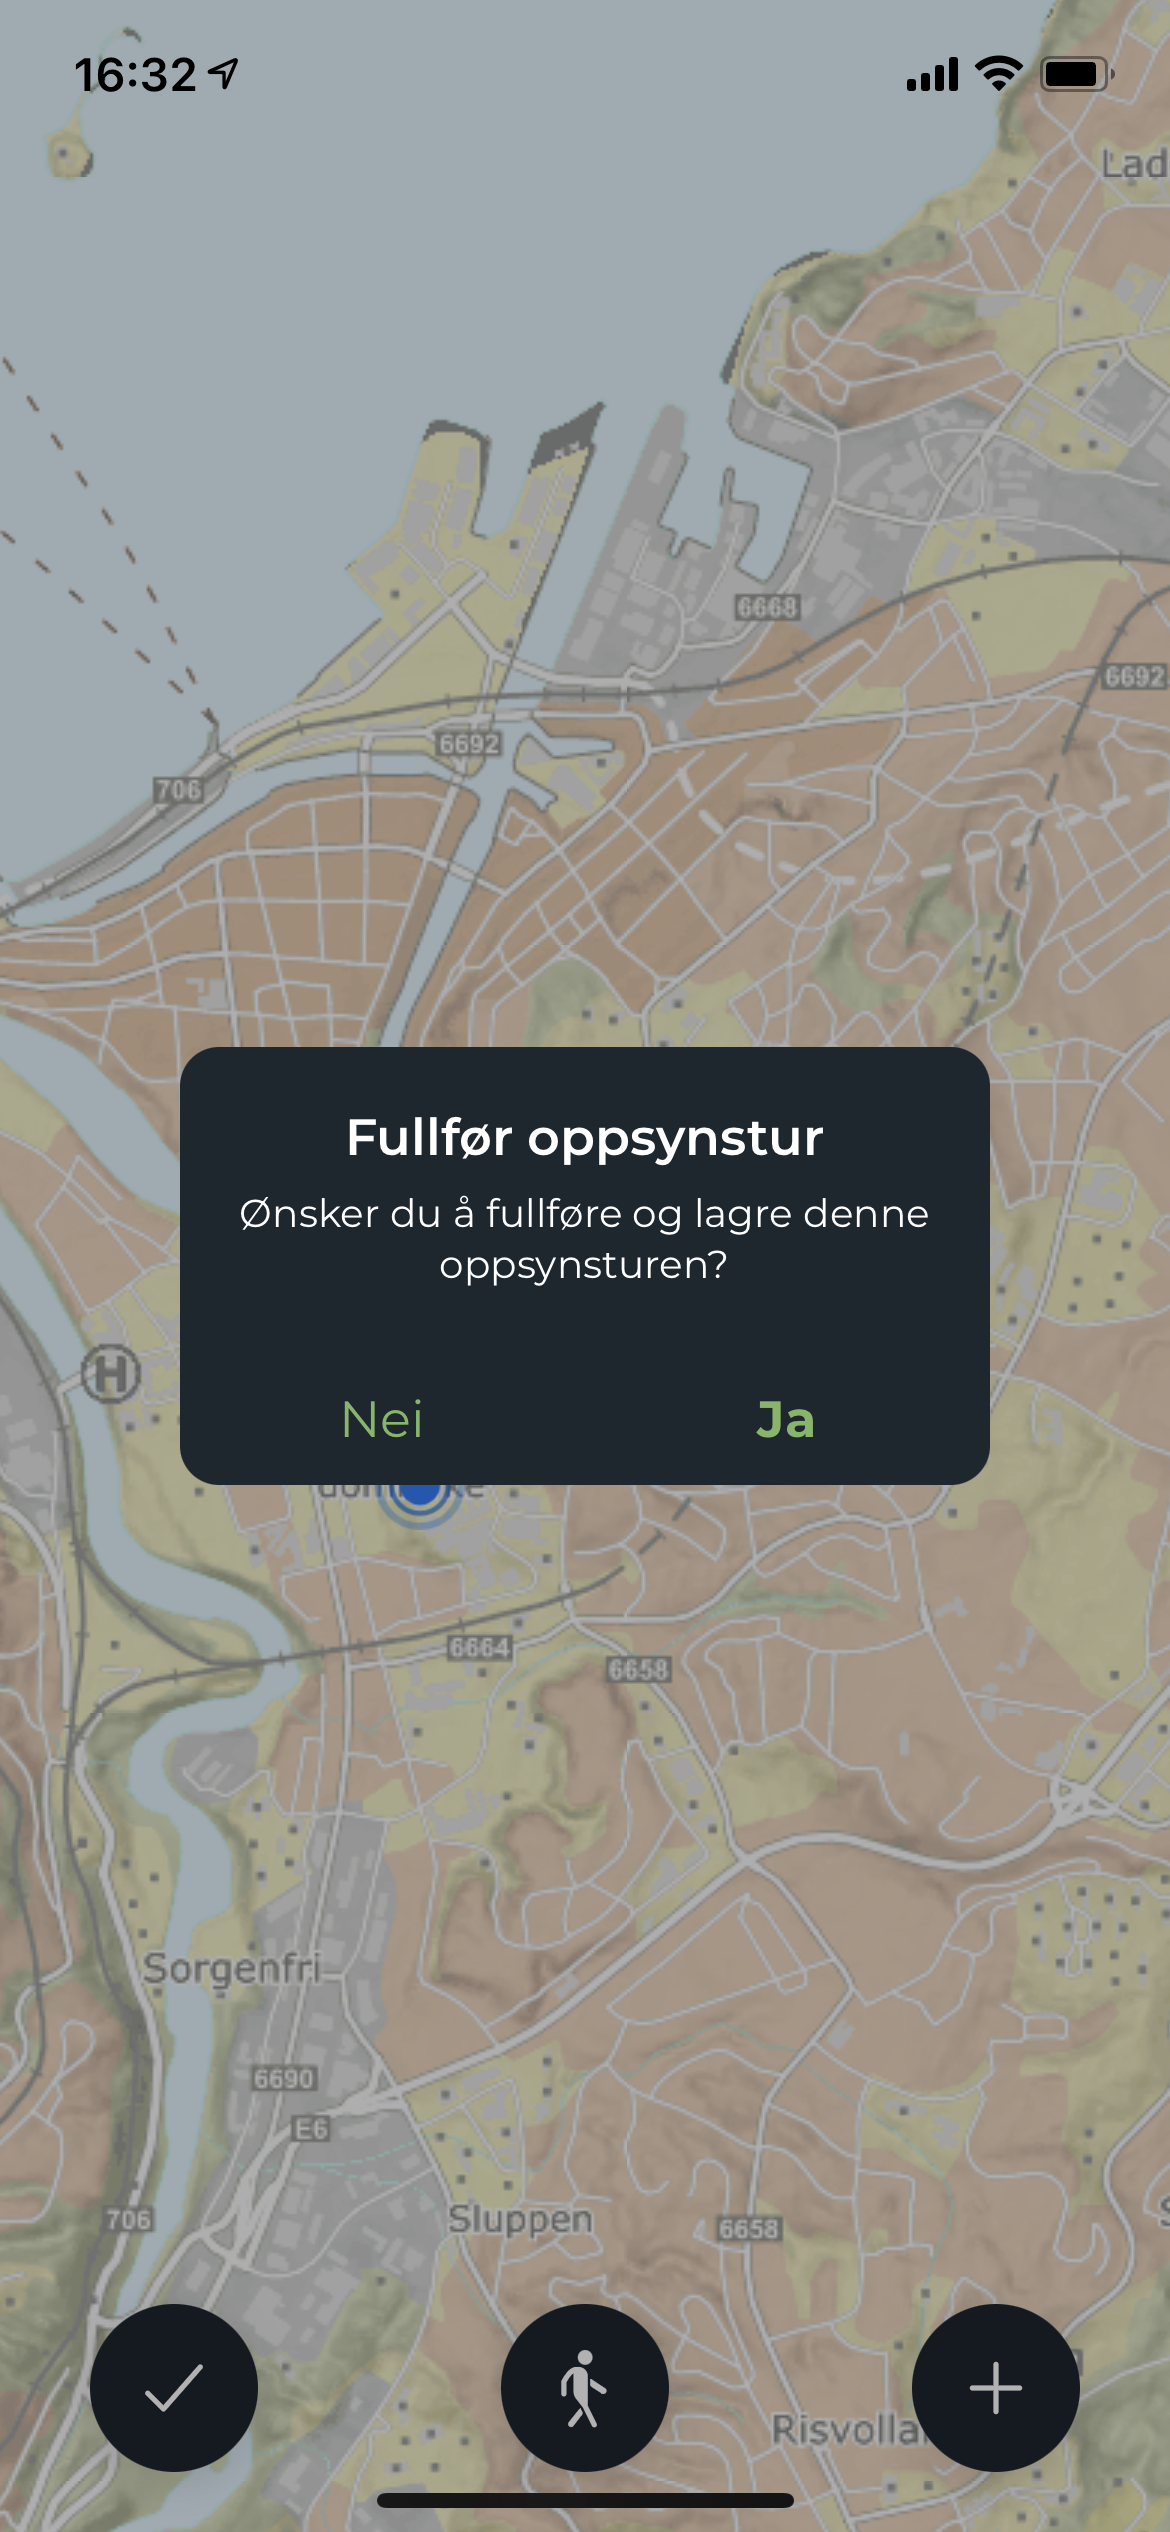
\includegraphics[scale=0.4]{Figurer/skjermbilder/follfore-oppsynstur.png}
    \caption{HER SKAL DET VÆRE ET BILDE AV EN FULLFØRT OPPSYNSTUR!.}
    \label{fig:oppsynstur-oppsummering}
  \end{minipage}
\end{figure}

\section{Bakgrunnoppdatering av GPS-lokasjon} \label{sec:bakgrunnsoppdatering-av-gps-lokasjon}
Det var opprinnelig tenkt å implementere bakgrunnsoppdatering av GPS-lokasjon under en registrering. Etter flere mislykkede forsøk på å implementere bakgrunnsoppdatering av GPS-lokasjon, endte det til slutt opp med å skrinlegge idéen og heller legge til en funksjon som ville gjøre det mulig å spare strøm mens applikasjonen kjører i forgrunnen. Ved å trykke på knappen nede i midten av kartgrensesnittet (se figur \ref{fig:registrert-rovdyr}), aktiveres gå-/strømsparings-modusen. Skjermen vil da bli svart, og en forklarende tekst som forteller hvordan man kommer seg ut av strømsparingsmodus vil vises fram før den forsvinner etter 8 sekunder. Ved å gjøre hele skjermen svart vil nyere mobilskjermer som tar i bruk OLED-teknologi kunne spare betydelig mengder strøm som ellers ville blitt brukt til å vise fram bilder på skjermen. I en undersøkelse gjort av Mian et al. \cite{dongPowersavingColorTransformation2009} utforskes bruk av mørke energisparende brukergrensesnitt for OLED-skjermer. Resultatene viser at det var mulig å bruke 75\% mindre strøm ved bruk av svarte og grønne grensesnitt framfor vanlige grensesnitt. Ettersom at applikasjonen vår viser fram en helt svart skjerm under gå-/strømsparings-modus tør vi å anta at dette tallet vil være enda høyere i vårt tilfelle.
\begin{figure}[H]
\centering
\captionsetup{width=.8\linewidth}
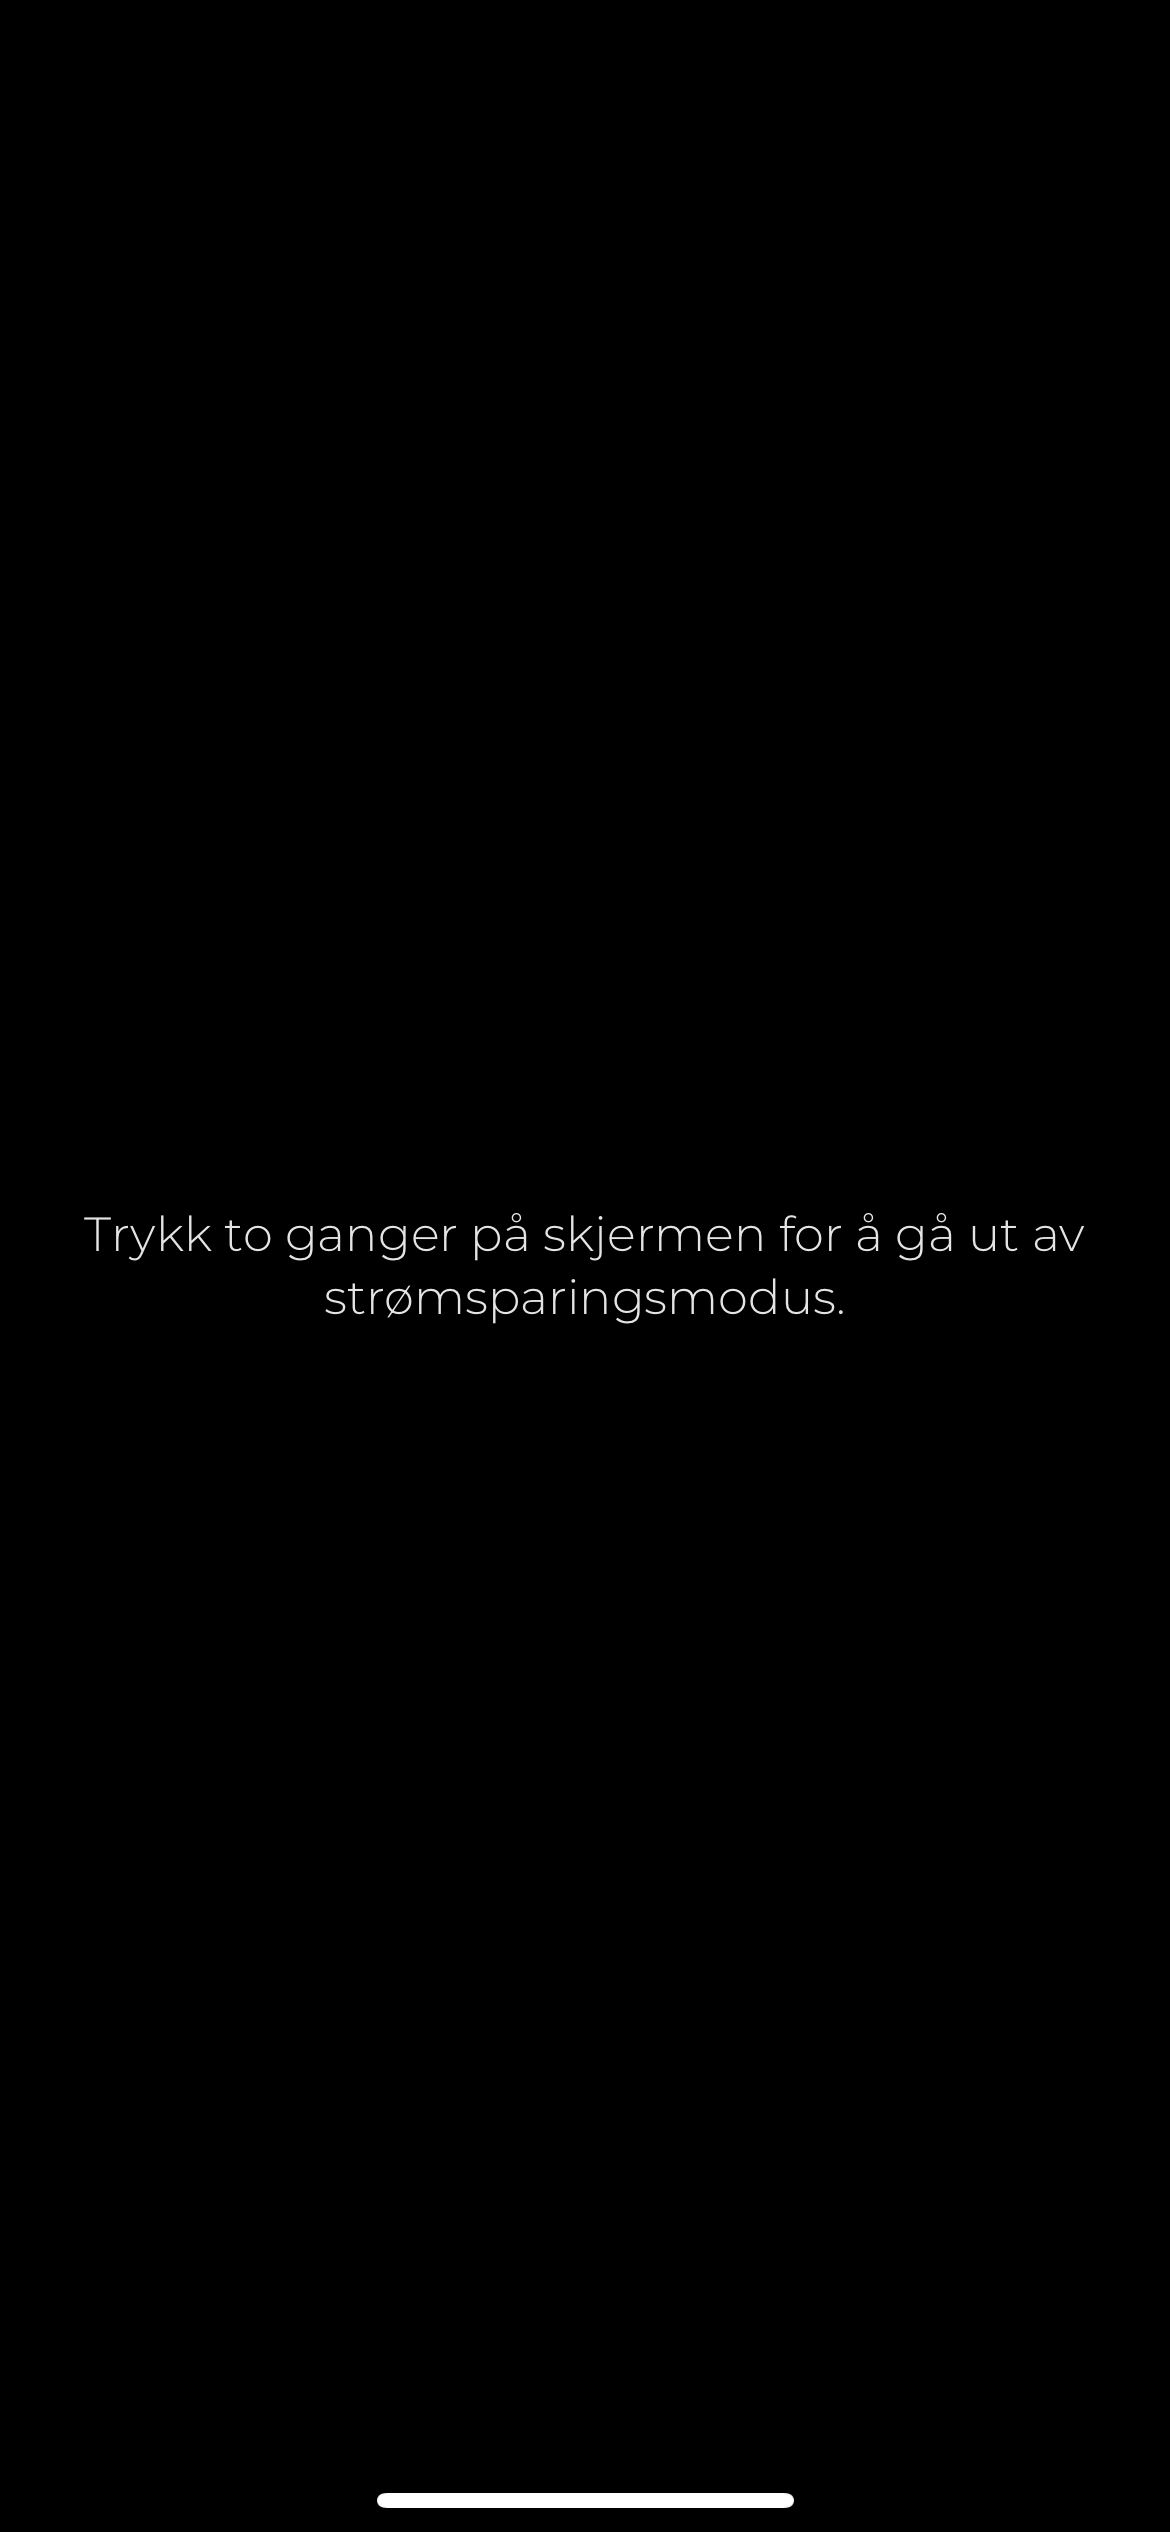
\includegraphics[scale=0.4]{Figurer/skjermbilder/stromsparing.png}
\caption{Skjermbilde av hvordan applikasjon ser ut rett etter at knappen for gå-/strømsparings-modus har blitt trykket på.}
\label{fig:stromsparing}
\end{figure}

\section{Tilstandshåndtering} \label{sec:tilstandshandtering}
For at applikasjonen skulle fungere som ønsket var det viktig å få på plass et solid tilstandshåndteringssystem. Med tilstandshåndtering menes det at man har programmatisk kontroll over tilstanden i applikasjonen og har mulighet til å lese eller endre denne. Hvis en del av applikasjonen endrer tilstanden, vil alle andre deler av applikasjonen få vite om dette. Tilstand kan, i vårt tilfellet, for eksempel være hvor mange søyer med grønt slips som har blitt registrert. Applikasjonen må til en hver tid å ha kontroll over hvor brukeren befinner seg i grensesnittet under registreringen av en saueflokk, samt hvilke registreringer som har blitt gjort for å kunne lese opp korrekt tekst til brukeren under en blind registrering. For å løse dette ble det bestemt å bruke NGXS. NGXS er et rammeverk og et bibliotek for tilstandshåndtering som er godt brukt og spesielt laget for Angular (NGXS omtales mer i underkapittel \ref{sub:ngxs} \nameref{sub:ngxs}). Tilstandshåndteringen for applikasjonen er delt i tre, hvor en del tar seg av hvilken kategori og underkategori brukeren er i under registrering av en saueflokk. En annen del tar seg av hvor mange sauer som har blitt registrert under hver underkategori, og den siste delen tar seg av alle registreringen som har blitt gjort for en hel oppsynstur.

\subsection{Tilstand for kategori og underkategori under registrering av saueflokk}
Tilstanden for kategori og underkategori under registrering av en saueflokk, kalt \textit{AppInfo.state} består av bare to verdier. En verdi som forteller hvilken underkategori brukeren befinner seg på (\textit{CurrentSubcategory}) og en som forteller hvilken hovedkategori brukeren befinner seg på (\textit{CurrentCategory}). \textit{AppInfo.state} inneholder også metoder for å endre og hente denne tilstanden og tilhørende informasjon.
\begin{figure}[H]
\centering
\captionsetup{width=.8\linewidth}
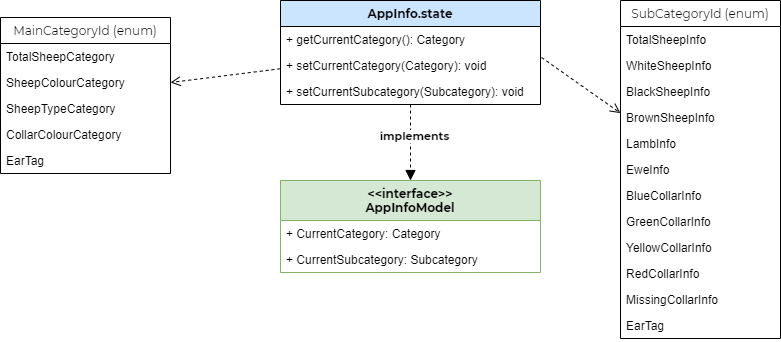
\includegraphics[scale=0.65]{Figurer/diagram/tilstand_registrering.png}
\caption{Klassediagram for tilstandshåndtering av kategori og underkategori under registrering av en saueflokk.}
\label{fig:tilstand_registrering}
\end{figure}

\subsection{Tilstand for registrering av en sauflokk}
Figur \ref{fig:tilstand_sau} viser et klassediagram for hvordan informasjonen for registreringen av en sauflokk blir delt inn i kategorier og underkategorier. Både klassen \textit{SubCategory} og \textit{MainCategory} implementerer interfacet \textit{Category}. Dette gjør det enkelt å utvide disse klassene om det skulle være nødvendig. Det samme kan man si om klassene \textit{TotalSheep}, \textit{SheepColour}, \textit{SheepType}, \textit{CollarColour} og \textit{EarTag} som alle arver fra \textit{MainCategory}. Målet med å utforme klassene på denne måten var å muliggjøre å enkelt kunne legge til enten nye kategorier eller underkategorier i framtiden.
\begin{figure}[H]
\centering
\captionsetup{width=.8\linewidth}
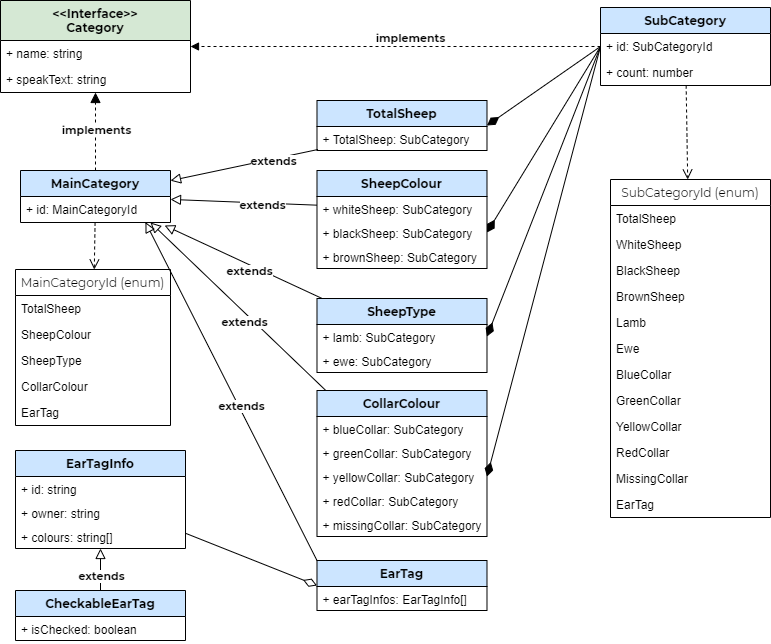
\includegraphics[scale=0.6]{Figurer/diagram/tilstand_sau.png}
\caption{Klassediagram for tilstandshåndtering av opptalte sauer del 1.}
\label{fig:tilstand_sau}
\end{figure}

\noindent
\textit{SheepInfo.state} vises i figur \ref{fig:tilstand_sau_state}. \textit{SheppInfo.state} inneholder tilstanden for all de fem hovedkategoriene, samt forskjellige metoder for å gjøre det enkelt å inkrementere eller dekrementere antallet registrerte for hver underkategori.

\begin{figure}[H]
\centering
\captionsetup{width=.8\linewidth}
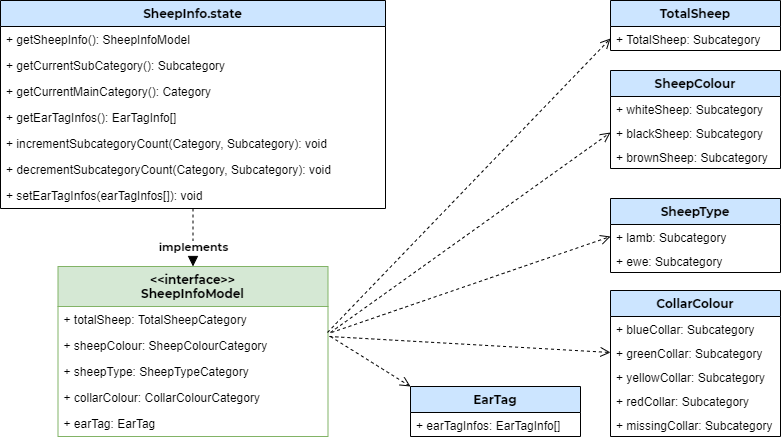
\includegraphics[scale=0.6]{Figurer/diagram/tilstand_sau_state).png}
\caption{Klassediagram for tilstandshåndtering av opptalte sauer del 2.}
\label{fig:tilstand_sau_state}
\end{figure}

\subsection{Tilstand for en oppsynstur}
I likhet med strukturen for registrering av en saueflokk er også strukturen for en oppsynstur laget modulært for å gjøre det mulig å for eksempel legge til en ny type registrering i framtiden. Klassen \textit{FieldTripInfo} innholder all informasjon som er nødvendig i forbindelse med en oppsynstur. Den inneholder også alle registreringer som er gjort i form av en liste med objekter av typen \textit{Registration}. Klassene \textit{SheepRegistration}, \textit{DeadSheepRegistration}, \textit{InjuredSheepRegistration} og \textit{PredatorRegistration} arver alle fra \textit{Registration}, noe som gjør det enkelt å legge til en ny type registrering om ønskelig. \textit{FieldTripInfo.state} inneholder én versjon av klassen \textit{FieldTripInfo}, samt metoder for å hente, oppdatere og legge til nye registreringer.
\begin{figure}[H]
\centering
\captionsetup{width=.8\linewidth}
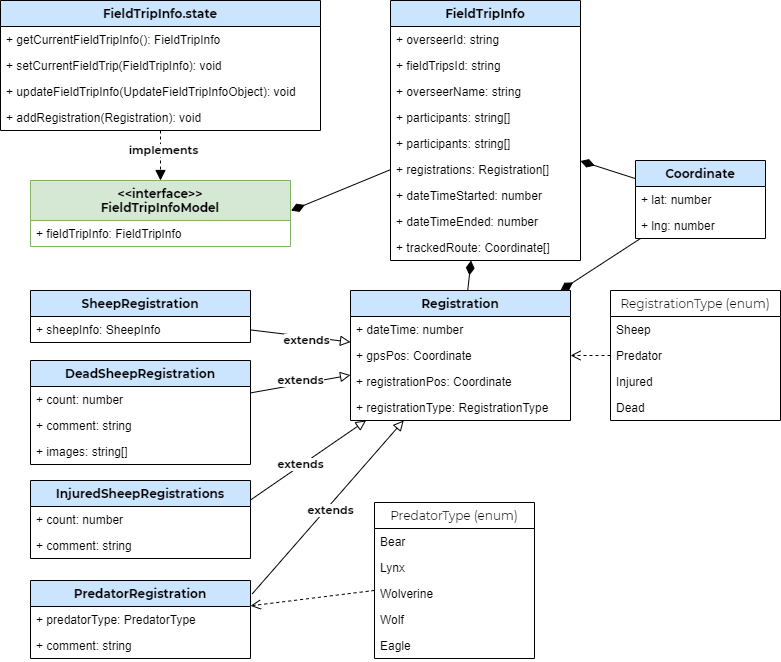
\includegraphics[scale=0.6]{Figurer/diagram/tilstand_oppsynstur.png}
\caption{Klassediagram for tilstandshåndtering av en oppsynstur.}
\label{fig:tilstand_oppsynstur}
\end{figure}


\section{Backend}
Framfor å bruke et mer tradisjonelt oppsett med en dedikert backend-tjener og tilhørende database, bruker applikasjonen Firebase som backend i form av Backend-as-a-Service. Ettersom at Firebase har løsninger for både autentisering, autorisering og database, betydde dette at vi kunne bruke mer tid på å implementere klient-delen av applikasjonen framfor å bruke tid på eventuell backend-logikk.

\subsection{Login} \label{sub:backend-login}
For innlogging brukes Firebase Authentication gjennom Firebase Cloud. Personer som har fått tildelt en bruker kan logge seg inn ved hjelp av e-post og passord. Firebase har løsninger som tillater innlogging ved hjelp av en tredjepart som for eksempel Google eller Facebook. Dette kan enkelt implementeres på et senere tidspunkt om ønskelig. Per dags dato kan nye brukere bare registreres av utviklere gjennom konsollen til Firebase.

\subsection{Database}
For lagring av data i forbindelse med applikasjonen brukes Firebase Cloud Firestore. Cloud Firestore er en dokumentdatabase hvor dokumenter lagres i samlinger kalt \textit{collections}. Databasen er delt opp i tre forskjellige samlinger; \textit{members}, \textit{beitelag} og \textit{fieldTrips}. Samlingen \textit{members} inneholder et dokument for hver bruker av applikasjonen med informasjon om id som er knyttet til Firebase Authentication, navn, beitelagId og e-postadresse. Samlingen \textit{beitelag} inneholder et dokument for hvert beitelag som registreres i applikasjonen. Per nå kan nye beitelag bare registreres av utviklere gjennom konsollen til Firebase. Et beitelag innholder fire forskjellige data; navn, bønder (\textit{farmers}), gjetere (\textit{overseers}) og oppsynsturer (\textit{fieldTrips}). Datafeltet \textit{farmers} inneholder en liste med ider over brukere som er registrert som bønder i et beitelag. En bonde vil ha tilgang til å se på alle oppsynsturer registrert av alle brukere for et beitelag. I motsetning til dette vil brukere registrert med sin id i \textit{overseers}-listen for et beitelag bare ha tilgang til å se oppsynsturer registrert av seg selv. Logikken for dette ligger i Firestore Security Rules og håndteres på tjenersiden av Firebase. Hvert beitelagsdokument peker til en egen \textit{fieldTrips}-samling som inneholder alle oppsynsturene som er registrert for det gitte beitelaget.

\begin{figure}[H] 
\centering
\captionsetup{width=.8\linewidth}
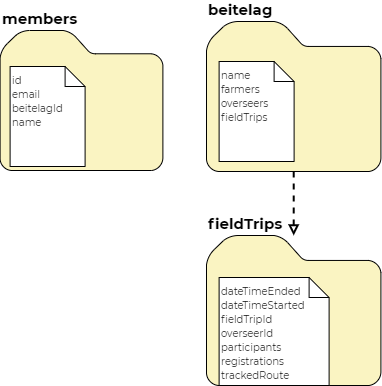
\includegraphics[scale=0.6]{Figurer/diagram/databasestruktur.png}
\caption{Databasestrukturen for Cloud Firestore.}
\label{fig:databasestruktur}
\end{figure}

\noindent
Figur \ref{fig:firebase_baas} viser en flyt for innlogging og registrering av en oppsynstur ved hjelp av Firebase. Når en bruker åpner applikasjonen på mobilen sin (klient) vil brukeren bli bedt om å oppgi brukernavn og passord. Dette sendes til Firebase Authentication som sjekker om opplysningene er korrekte og deretter gir brukeren tilgang til applikasjonen. Når brukeren skal laste opp en oppsynstur går kallet gjennom Firestore Security Rules. Her sjekkes det som brukeren er logget inn, om oppsynsturen inneholder alle nødvendige data og om brukeren er den den oppgir seg for å være og er registrert i det oppgitte beitelaget. Om alt er som det skal lagres oppsynsturen i Cloud Firestore som et dokument i \textit{beitelag}-samlingen. En bekreftelse sendes deretter tilbake til brukeren og forteller om alt gikk som den skulle.

\begin{figure}[H] 
\centering
\captionsetup{width=.8\linewidth}
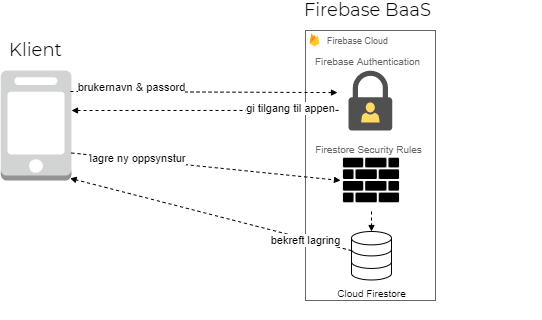
\includegraphics[scale=0.8]{Figurer/diagram/firebase_baas.png}
\caption{Diagrammet viser interaksjon mellom BaaS og en klient for innlogging og lagring av en ny oppsynstur.}
\label{fig:firebase_baas}
\end{figure}


\section{Konklusjon}

\noindent
Løsningen som har blitt implementert for å muliggjøre bruk av offline-kart møter kravet F1 spesifisert i kravspesifikasjonen (se tabell \ref{tbl:funksjonelle-krav}). F1 sier at kartet skal ta i bruk Kartverkets tjenester i form av NorgesKart. Dette kravet innfris ved bruk av cache-tjenesten til Geonorge, som er utviklet av Kartverket. Krav F1 spesifiserer også at brukeren skal ha tilgang til de mest oppdaterte kartbildene. Dette løses ved at det er mulig å oppdatere et kartutsnitt enkelt gjennom grensesnittet som vist ved \enquote{Oppdater}-knappen i figur \ref{fig:nedlastede-kartutsnitt-apen-meny}. Løsningen tilfredsstiller også det funksjonelle kravet F1.1 (se tabell \ref{tbl:funksjonelle-krav}), som sier at brukeren skal kunne laste ned et kartutsnitt som skal kunne benyttes når mobilen ikke har tilgang på internett. Det har blitt implementert funksjonalitet for å vise fram brukerens rute, samt mulighet for å registrere observasjoner i form av pins på kartet. Dette oppfyller de funksjonelle kravene F1.2 og F1.3. Alle krav og underkrav for F2 har blitt innfridd. All nødvendig informasjon som farge på sau, slips, øremerker og om de er søye eller lam kan registreres om brukeren ønsker det. Nye øremerker kan legges til med navn på tilhørende bonde og inntil to forskjellige farger. Når en oppsynstur avsluttes gis det tilbakemeldinger på om det har oppstått avvik i registreringen av en saueflokk. Registreringer lagres også eksternt i Firebase Cloud Firestore, noe som gjør det mulig å dele oppsynsturer med alle i samme beitelag. Kravet F3, \textit{Systemet skal ha innlogging med brukernavn og passord} har blitt nådd ved hjelp av Firebase Authentication. Kravet F1.3, \textit{Brukeren skal ha egen profil og mulighet til å se og endre på den}, har ikke blitt implementert da dette ikke ble sett på som viktig nok funksjonalitet. Alle krav og underkrav for F4 ble innfridd allerede under fordypningsprosjektet.
\newline
\newline
\noindent
 De ikke-funksjonelle kravene har IF1, \textit{Applikasjonen skal fungere uten internett} og IF2, \textit{Applikasjonen skal være kryssplattform ...} har blitt oppnådd. Kravet IF3 har ikke blitt testet i denne omgang. Kravet IF4 ble testet i fordypningsprosjektet, hvor det kom fram at en kombinasjon av haptisk tilbakemelding, tekstopplesing, samt interaksjon gjennom sveiping og trykking på grensesnittet for blind registrering var det mest effektive.